\documentclass{book}
\usepackage[utf8]{inputenc}
\usepackage{amssymb}
\usepackage{amsmath}
\usepackage{graphicx}
\usepackage{mathpartir}
\usepackage[margin=1.5in]{geometry}
\usepackage{verbatim}
\usepackage{subfig}
\usepackage{wrapfig}
\usepackage{float}
\usepackage{pgfplots}
\usepackage{bold-extra}
\usepackage{tikz}
\usepackage{palatino}
\usepackage[T1]{fontenc}
\usepackage{inconsolata}
\usepackage{natbib}
\usepackage{longtable}
\usepackage{tikz}
\usepackage{array}
%\usepackage{graphicx}
%\usepackage[table]{xcolor}
\usepackage{colortbl}
%\usepackage{url}
\usepackage[pdfborder=0 0 0]{hyperref}
\hypersetup{
    colorlinks,
    linkcolor=black,
    citecolor=black,
    filecolor=black,
    urlcolor=black
}
\usepackage{xparse}
\usepackage{enumitem}  % sensible enumerations
\setlist{nolistsep}

%\usepackage{parskip}
%\setlength{\parindent}{-0.0cm}
%\setlength{\parskip}{0.3\baselineskip}


%\usepackage[compact]{titlesec}

%\usepackage{titlesec}
%\titleformat{\chapter}[hang]{\huge}{\thechapter}{1em}{}
%\titlespacing{\chapter}{0pt}{0pt}{0cm}

\let\cleardoublepage\clearpage

\usepackage{fancyheadings}
\pagestyle{fancy}
%\addtolength{\headwidth}{\marginparsep}
%\addtolength{\headwidth}{\marginparwidth}
\renewcommand{\chaptermark}[1]{\markboth{#1}{}}
\renewcommand{\sectionmark}[1]{\markright{\thesection\ #1}}
\lhead[\fancyplain{}{\bfseries\thepage}]
{\fancyplain{}{\bfseries\rightmark}}
\rhead[\fancyplain{}{\bfseries\leftmark}]
{\fancyplain{}{\bfseries\thepage}}
\cfoot{}

\usepackage{listings}

\lstnewenvironment{code}[1][]%
  {
   \noindent
   \minipage{\linewidth}
   \vspace{0.2\baselineskip}
%   \vspace{-0.4\baselineskip}
   \lstset{basicstyle=\ttfamily\footnotesize,
           frame=single,
           language=Haskell,
           keywordstyle=\color{black},
           #1}}
  {%\vspace{-0.8\baselineskip}
   \endminipage}

\makeatletter
\newcommand*{\rom}[1]{\text{\footnotesize\expandafter\@slowromancap\romannumeral #1@.}}
\newcommand*{\romnodot}[1]{\text{\footnotesize\expandafter\@slowromancap\romannumeral #1@}}
\makeatother

%\newcommand\note[1]{\mbox{}\marginpar{\footnotesize\raggedright\hspace{0pt}\emph{#1}}}
\newcommand\note[1]{}
\newcommand\PA{\mathcal{P\!A}}
\newcommand\hs[1]{\texttt{#1}}
\newcommand\ts[1]{\texttt{#1}}
\newcommand\fn[1]{\mathrm{#1}}
\newcommand\ptr[1]{\fn{#1.ptr}}
\newcommand\appfn{@}
\newcommand\app[2]{#1 \, \appfn \, #2}
\newcommand\ex[1]{\exists \, #1 \, . \,}
\newcommand\nexxx[3]{\nexists \, #1 , #2 , #3 . \,}
\newcommand\fa[1]{\forall \, #1 . \,}
\newcommand\faa[2]{\forall \, #1 , #2 . \,}
\newcommand\faaa[3]{\forall \, #1 , #2 , #3 . \,}
\newcommand\faaaaaa[6]{\forall \, #1 , #2 , #3 , #4 , #5 , #6 . \,}

\newcommand{\HRule}{\rule{\linewidth}{0.5mm}}%\usetikzlibrary {\trees,positioning,arrows}

\newcommand\tofix[1]{\fixb{#1}}
\newcommand\unfix[1]{\fixw{#1}}

\newcommand\fixb[1]{#1^{\bullet}}
\newcommand\fixw[1]{#1^{\circ}}

\newcommand\fixhsb[1]{\hs{#1}^{\bullet}}
\newcommand\fixhsw[1]{\hs{#1}^{\circ}}

\newcommand\append[0]{\texttt{\small{++}}}

\newcommand{\xsys}[2]{#1 \, xs \, #2 & = #1 \, ys #2}
\newcommand{\desca}[1]{  & \hspace{44.5mm}                            \{ \text{#1} \}}
\newcommand{\descra}[1]{ & \hspace{35mm} \Rightarrow     \hspace{4mm} \{ \text{#1} \}}
\newcommand{\descla}[1]{ & \hspace{35mm} \Leftarrow      \hspace{4mm} \{ \text{#1} \}}
\newcommand{\desclra}[1]{& \hspace{35mm} \Leftrightarrow \hspace{4mm} \{ \text{#1} \}}

\newcommand\lub[1]{\sqcup_{#1}}
\newcommand\defof[1]{definition of #1}

\newcommand\w[0]{\,\,}
\newcommand\eq[0]{ = }

\newcommand{\defBNF}[4] {\text{#1}\quad&#2&::=&\;#3&\text{#4}}
\newcommand{\defaltBNF}[2] {&&|&\;#1&\text{#2}}

\newcommand{\hstup}[2]{\hs{(} #1 \hs{,} #2 \hs{)}}

\newcommand{\nsqsubseteq}{\,\,\, /\!\!\!\!\!\!\sqsubseteq}

%\begin{document}
%
%\chapter{Introduction}
%
%
\chapter{Introduction}


Consider this data type of trees \citep{grafting} and its implementation
of \hs{Monad} \citep{mtl}:

\begin{code}
data Tree a = Fork (Tree a) (Tree a) | Leaf a

return :: a -> Tree a
return = Leaf

(>>=) :: Tree a -> (a -> Tree b) -> Tree b
Fork u v >>= f = Fork (u >>= f) (v >>= f)
Leaf x   >>= f = f x
\end{code}

\noindent
Could the elegant simplicity of bind possibly obey the three monad
laws as stated by \cite{essenceoffp}? Referential transparency in
Haskell allows equational reasoning, but proving the monad laws by
hand can be tiresome. This is a situation where our tool can help:
write down the equations in a similar style as properties in
QuickCheck \citep{quickcheck}. Run the tool on the source file which
reports this after a few seconds\footnote{The presentation format is
  slightly rewritten for your viewing pleasure.}:


\begin{code}
Theorems (3/3):
  prop_return_right: t >>= return == t
    by structural induction on t and by approximation lemma

  prop_return_left: return x >>= f == f x
    by definitional equality and by approximation lemma

  prop_assoc: (t >>= f) >>= g == t >>= (\x -> f x >>= g)
    by structural induction on t and by fixed point induction on (>>=)
\end{code}

\noindent
The output \hs{Theorem} means that the properties hold for infinite
trees, in contrast to the possible result \hs{Finite Theorem}.

What is going on behind the scenes to prove this? The key components
of this tool are:

\begin{enumerate}
{\setlength\itemindent{18pt} \item a translation from Haskell to \emph{first order logic},}
{\setlength\itemindent{18pt} \item instantiating the properties with different \emph{induction techniques}, and}
{\setlength\itemindent{18pt} \item running \emph{automated theorem provers} on the generated theories.}
\end{enumerate}
The technology described and discussed in this thesis allows an
automated way to prove \emph{equational properties}. Moreover, it can
reason about \emph{infinite values} as the \hs{Tree}s above.

\section{Aim}

The aim of this thesis is to develop a tool able to do automated
proving of Haskell properties. This should be realised by means of
different induction techniques, a translation to first order logic and
invocations to automated theorem provers. The tool should be able to
reason and prove properties about lazy data structures, higher order
functions and infinite and partial values. The project is restricted
to equational properties to keep it tractable, and equality should
coincide with equality in first order logic. This means that two
values are equal if they are created by the same constructor, and the
arguments to the constructors are all equal.

\section{Background}

To read this thesis, the reader should have at least brief knowledge
of Haskell. An introduction is given by \cite{lyah}. Some familiarity
of model theory and proof deduction in first order logic is
beneficial, as well as a grasp of proofs by induction. At least a
shallow apprehension of using automated theorem provers is assumed.
The rest of this thesis should be self contained.











































\begin{comment}
INTRODUCTION - State your thesis and the purpose of your research
paper clearly. What is the chief reason you are writing the paper?
State also how you plan to approach your topic. Is this a factual
report, a book review, a comparison, or an analysis of a problem?
Explain briefly the major points you plan to cover in your paper and
why readers should be interested in your topic.
\end{comment}



\begin{comment}

%% Shit the same, just write something

%In this thesis we introduce a new way to automatically prove
%properties of Haskell programs with the aid of automated theorem
%provers (ATPs).

Haskell is celebrated for being a language easy to reason about.
Referential transparency makes equational reasoning easy and
sound. The testing tool QuickCheck \citep{quickcheck} has influenced
programmers to state properties about their program's functions. This
thesis introduces an automated way to prove properties with the aid of
automated theorem provers, by means of a translation from Haskell to
First Order Logic. This compilation can handle the important concepts
of higher order functions and lambda abstraction, and can deal with
infinite values as well as partial values from pattern match failures
or partial functions.

We currently handle universally quantified equational properties. From
the programmers perspective, they can be entered in the source code
like this:

\begin{code}
prop_filter_append :: (a -> Bool) -> [a] -> [a] -> Prop [a]
prop_filter_append p xs ys = filter p (xs ++ ys) =:= filter p xs ++ filter p ys
\end{code}

\noindent
Every function and data definition needs to be translated into a
theory in first order logic which we can call $\mathcal{T}$. The
property above then corresponds to this proving this:

\begin{equation*}
\mathcal{T} \vdash \faaa{p}{xs}{ys} \fn{filter}(p,xs \,\append\, ys) = \fn{filter}(p,xs) \,\append\, \fn{filter}(p,ys)
\end{equation*}

\noindent
By writing $\fn{filter}$ and $\append$, it is emphasised that these
are the translations of \hs{filter} and \hs{++} axiomatised in
$\mathcal{T}$. To proceed to prove a property like this different
proving techniques for functional programs are automatically
tested. These can deal with reasoning about programs with both finite
arguments and infinite.

There are many examples of equality properties.  Verifying that an
efficient and a naive implementation solution coincide. Proving
fundamental laws that your functions should hold, be it the axioms of
a ring, or more specifically, idempotency of sorting or involution of
reversing, or relating different functions in terms of homomorphisms
or more complicated relations. The rich plethora of type classes in
Haskell have many stipulated equational laws.

Equality is between Haskell values, and not the different equalities
defined by the \hs{Eq} type class. It is however possible to express
such properties as well. One example is the relation between
\hs{lookup} and \hs{adjust} from \hs{Data.Map} in the containers
package:

\begin{code}
prop_lookup_alter :: (Maybe a -> Maybe a) -> k -> Map k a -> Map k a
prop_lookup_alter f k m = lookup k (alter f k m) == f (lookup k m) =:= True
\end{code}


\end{comment}

\begin{comment}

Why is equality important? There are many reasons why you would want
to know why two Haskell expressions are equal. You might have a naive
way of implementing an algorithm, and an efficient way, and you want
to know that those two implementations behave equally. Your functions
may be a familiar algebraic structure: monoid, group, ring, lattice
and so on, and you want to know that your implementation satisfies all
laws, or your functions may not have such a rich structure but still
have a lot of properties, like idempotency: sorting twice is the same
as sorting one, involution: reversing twice is the same as doing
nothing (but only for finite lists!). Functions could also be
homomorphisms over structures:
\hs{length (xs ++ ys)}$\eq$\hs{length xs + length xs} is an example of
a monoid homomorphism between list concatenation and addition. Haskell
is also known for its type classes like Functor, Applicative and
Monad, and all instances of these should satisfy certain equational
laws.

What is equality? In the general context, a binary relation is an
equivalence relation if it is reflexive ($\fa{x} x \eq x$), symmetric
($\faa{x}{y} x \eq y \rightarrow y \eq x$) and transitive
($\faaa{x}{y}{z} x \eq y \wedge y \eq z \rightarrow x \eq z$). In
Haskell, it is indeed so that every data type can have its own
instance of the \hs{Eq} type class, gives a computable function given
two values of the type and determines if they are equal, the result
given as true or false in a \hs{Bool}. In this project we have made
the simplification that two Haskell values are equal if they have
exactly the same structure: the same constructor at every depth. We
also regard the undefined value $\bot$ as a constructor, so
$\hs{x:}\bot$ is not equal to $\hs{x:[]}$. If the concept of $\bot$ is
unfamiliar to you, do not fear: it will be explained in great
detail. The reason for this simplification is that it will coincide
exactly with the equality in first order logic and allows us to use its
substitution.
\note{Congruence relations!}

\end{comment}
%
%\bibliographystyle{apalikeurl}
%\bibliography{masterbib}
%
%\end{document}
%
%\begin{comment}

\begin{document}

%% Title ----------------------------------------------------------------------
%\title{Proving Equational Haskell Properties Using Automated Theorem Provers}
%\author{Dan Rosén}
%\date{\today}
%\maketitle
\begin{titlepage}

\begin{center}


% Upper part of the page
%\includegraphics[width=0.15\textwidth]{./logo}\\[1cm]

\vspace{4cm}

\textsc{\LARGE University of Gothenburg}\\[1.5cm]

\textsc{\Large Master's Thesis}\\[0.5cm]


% Title
\HRule \\[0.4cm]
{ \huge \bfseries Proving Equational Haskell Properties Using Automated Theorem Provers}\\[0.3cm]

\HRule \\[1.5cm]

% Author and supervisor
\begin{minipage}{0.4\textwidth}
\begin{flushleft} \large
\emph{Author:}\\
Dan Rosén
\end{flushleft}
\end{minipage}
\begin{minipage}{0.4\textwidth}
\begin{flushright} \large
\emph{Supervisor:} \\
Koen Claessen
\end{flushright}
\end{minipage}

\vfill

% Bottom of the page
{
\Large \textbf{DRAFT}

\vspace{2cm}

\large \today
}

\end{center}

\end{titlepage}

%% Abstract -------------------------------------------------------------------

\thispagestyle{empty}

\section*{\centering \begin{normalsize}Abstract\end{normalsize}}

\begin{quotation}
\noindent
This Master thesis gives a new tool to automatically verify equational
properties written in the functional programming language Haskell,
with the aim to be able to reason about infinite and partial values
available in Haskell from general recursion and lazy data
structures. The novelty of this approach is to use automated theorem
provers for first order logic by means of a translation from Haskell
to first order theories. The properties are instantiated with
different induction techniques applicable to non strict functional
languages: structural induction, fixed point induction and the
approximation lemma. As the target logic is untyped, Haskell features
such as pattern matching and higher order functions needs to be dealt
with special care. The results from using the tool on a test suite are
convincing as the automated provers quickly deduce theorems for a
variety of properties. To be able to compete on fair grounds with
contemporary tools a system for adding lemmas would be required, which
turned out to be difficult as theorems for finite and infinite values
do not coexist peacefully out of the box.
\end{quotation}



%% Acknowledgements -----------------------------------------------------------

%\newpage
%\pagestyle{empty}
%\section*{Acknowledgments}
%\vspace{5mm}
%ACK, ACK, ACK, ACK, ACK, ACK, NAK

%% Table of Contents ----------------------------------------------------------

\newpage
\tableofcontents
\addtocontents{toc}{\protect\thispagestyle{empty}}

\newpage
\setcounter{page}{1}


\chapter{Introduction}


Consider this data type of trees \citep{grafting} and its implementation
of \hs{Monad} \citep{mtl}:

\begin{code}
data Tree a = Fork (Tree a) (Tree a) | Leaf a

return :: a -> Tree a
return = Leaf

(>>=) :: Tree a -> (a -> Tree b) -> Tree b
Fork u v >>= f = Fork (u >>= f) (v >>= f)
Leaf x   >>= f = f x
\end{code}

\noindent
Could the elegant simplicity of bind possibly obey the three monad
laws as stated by \cite{essenceoffp}? Referential transparency in
Haskell allows equational reasoning, but proving the monad laws by
hand can be tiresome. This is a situation where our tool can help:
write down the equations in a similar style as properties in
QuickCheck \citep{quickcheck}. Run the tool on the source file which
reports this after a few seconds\footnote{The presentation format is
  slightly rewritten for your viewing pleasure.}:


\begin{code}
Theorems (3/3):
  prop_return_right: t >>= return == t
    by structural induction on t and by approximation lemma

  prop_return_left: return x >>= f == f x
    by definitional equality and by approximation lemma

  prop_assoc: (t >>= f) >>= g == t >>= (\x -> f x >>= g)
    by structural induction on t and by fixed point induction on (>>=)
\end{code}

\noindent
The output \hs{Theorem} means that the properties hold for infinite
trees, in contrast to the possible result \hs{Finite Theorem}.

What is going on behind the scenes to prove this? The key components
of this tool are:

\begin{enumerate}
{\setlength\itemindent{18pt} \item a translation from Haskell to \emph{first order logic},}
{\setlength\itemindent{18pt} \item instantiating the properties with different \emph{induction techniques}, and}
{\setlength\itemindent{18pt} \item running \emph{automated theorem provers} on the generated theories.}
\end{enumerate}
The technology described and discussed in this thesis allows an
automated way to prove \emph{equational properties}. Moreover, it can
reason about \emph{infinite values} as the \hs{Tree}s above.

\section{Aim}

The aim of this thesis is to develop a tool able to do automated
proving of Haskell properties. This should be realised by means of
different induction techniques, a translation to first order logic and
invocations to automated theorem provers. The tool should be able to
reason and prove properties about lazy data structures, higher order
functions and infinite and partial values. The project is restricted
to equational properties to keep it tractable, and equality should
coincide with equality in first order logic. This means that two
values are equal if they are created by the same constructor, and the
arguments to the constructors are all equal.

\section{Background}

To read this thesis, the reader should have at least brief knowledge
of Haskell. An introduction is given by \cite{lyah}. Some familiarity
of model theory and proof deduction in first order logic is
beneficial, as well as a grasp of proofs by induction. At least a
shallow apprehension of using automated theorem provers is assumed.
The rest of this thesis should be self contained.











































\begin{comment}
INTRODUCTION - State your thesis and the purpose of your research
paper clearly. What is the chief reason you are writing the paper?
State also how you plan to approach your topic. Is this a factual
report, a book review, a comparison, or an analysis of a problem?
Explain briefly the major points you plan to cover in your paper and
why readers should be interested in your topic.
\end{comment}



\begin{comment}

%% Shit the same, just write something

%In this thesis we introduce a new way to automatically prove
%properties of Haskell programs with the aid of automated theorem
%provers (ATPs).

Haskell is celebrated for being a language easy to reason about.
Referential transparency makes equational reasoning easy and
sound. The testing tool QuickCheck \citep{quickcheck} has influenced
programmers to state properties about their program's functions. This
thesis introduces an automated way to prove properties with the aid of
automated theorem provers, by means of a translation from Haskell to
First Order Logic. This compilation can handle the important concepts
of higher order functions and lambda abstraction, and can deal with
infinite values as well as partial values from pattern match failures
or partial functions.

We currently handle universally quantified equational properties. From
the programmers perspective, they can be entered in the source code
like this:

\begin{code}
prop_filter_append :: (a -> Bool) -> [a] -> [a] -> Prop [a]
prop_filter_append p xs ys = filter p (xs ++ ys) =:= filter p xs ++ filter p ys
\end{code}

\noindent
Every function and data definition needs to be translated into a
theory in first order logic which we can call $\mathcal{T}$. The
property above then corresponds to this proving this:

\begin{equation*}
\mathcal{T} \vdash \faaa{p}{xs}{ys} \fn{filter}(p,xs \,\append\, ys) = \fn{filter}(p,xs) \,\append\, \fn{filter}(p,ys)
\end{equation*}

\noindent
By writing $\fn{filter}$ and $\append$, it is emphasised that these
are the translations of \hs{filter} and \hs{++} axiomatised in
$\mathcal{T}$. To proceed to prove a property like this different
proving techniques for functional programs are automatically
tested. These can deal with reasoning about programs with both finite
arguments and infinite.

There are many examples of equality properties.  Verifying that an
efficient and a naive implementation solution coincide. Proving
fundamental laws that your functions should hold, be it the axioms of
a ring, or more specifically, idempotency of sorting or involution of
reversing, or relating different functions in terms of homomorphisms
or more complicated relations. The rich plethora of type classes in
Haskell have many stipulated equational laws.

Equality is between Haskell values, and not the different equalities
defined by the \hs{Eq} type class. It is however possible to express
such properties as well. One example is the relation between
\hs{lookup} and \hs{adjust} from \hs{Data.Map} in the containers
package:

\begin{code}
prop_lookup_alter :: (Maybe a -> Maybe a) -> k -> Map k a -> Map k a
prop_lookup_alter f k m = lookup k (alter f k m) == f (lookup k m) =:= True
\end{code}


\end{comment}

\begin{comment}

Why is equality important? There are many reasons why you would want
to know why two Haskell expressions are equal. You might have a naive
way of implementing an algorithm, and an efficient way, and you want
to know that those two implementations behave equally. Your functions
may be a familiar algebraic structure: monoid, group, ring, lattice
and so on, and you want to know that your implementation satisfies all
laws, or your functions may not have such a rich structure but still
have a lot of properties, like idempotency: sorting twice is the same
as sorting one, involution: reversing twice is the same as doing
nothing (but only for finite lists!). Functions could also be
homomorphisms over structures:
\hs{length (xs ++ ys)}$\eq$\hs{length xs + length xs} is an example of
a monoid homomorphism between list concatenation and addition. Haskell
is also known for its type classes like Functor, Applicative and
Monad, and all instances of these should satisfy certain equational
laws.

What is equality? In the general context, a binary relation is an
equivalence relation if it is reflexive ($\fa{x} x \eq x$), symmetric
($\faa{x}{y} x \eq y \rightarrow y \eq x$) and transitive
($\faaa{x}{y}{z} x \eq y \wedge y \eq z \rightarrow x \eq z$). In
Haskell, it is indeed so that every data type can have its own
instance of the \hs{Eq} type class, gives a computable function given
two values of the type and determines if they are equal, the result
given as true or false in a \hs{Bool}. In this project we have made
the simplification that two Haskell values are equal if they have
exactly the same structure: the same constructor at every depth. We
also regard the undefined value $\bot$ as a constructor, so
$\hs{x:}\bot$ is not equal to $\hs{x:[]}$. If the concept of $\bot$ is
unfamiliar to you, do not fear: it will be explained in great
detail. The reason for this simplification is that it will coincide
exactly with the equality in first order logic and allows us to use its
substitution.
\note{Congruence relations!}

\end{comment}

% Related work
\section{Related Work}

Zeno \citep{zeno} is the most similar work to this, proving equational
properties for Haskell programs. While Zeno supports type classes, and
implications with equational antecedents, and can generalize goals, it
makes no attempt to tackle infinite and partial values. Indeed, the
authors even ask themselves if it is not really a ML theorem prover.

%\note{Discuss this with Moa and get references}
Zeno translates its
proofs to Isabelle, which could maybe be described as a framework for
different logics: its most prominent use is as a theorem prover for
Higher Order Logic, commonly abbreviated Isabelle/HOL
\citep{isabelbook}. Different automated proving techniques has been
implemented, most notably the heuristic Rippling \citep{dixonphd},
found in IsaPlanner \citep{isaplanner}, which also relies on critics
\citep{productiveuse}. You can also call first order logic theorem
provers from Isabelle/HOL with Sledgehammer.

The proof assistant and programming language Coq resembles Isabelle in
the sense that each data type declaration generates an induction
principle and the user can write own induction procedures should it be
too weak. Coq has is quite automated in its use of tactics to resolve
goals, and has an own language Ltac to write such tactics, and a
rippling tactic has been implemented \citep{automateddtfp},
\citep{inductioncoq}.

Coq has some support for corecursion, and so has the dependently
language Agda \citep{norell:thesis}, whose strong type system based on
Martin-Löf type theory \citep{mltt} with inductive families, makes it a proof
assistant thanks to the Curry-Howard-Lambek correspondence. Its
support for corecursion has been investigated \citep{productivity},
although all of it is manual.

Effort has been put into automating the proof generation in Agda,
notably by \cite{agdaatp}, which is quite alike this work in its
translation from Agda to first order logic. One must however give
quite much information to the theorem prover, like how to instantiate
the induction hypotheses. %\note{Peter Dybjer maybe said that it could be seen as a very nice way to interact with a theorem prover, thanks to Agda.}
A more constructive approach by \cite{dtatp}, where they
do not only make calls to the Waldmeister theorem prover to assert
proof's truth, but they also translate the prover's output back to
functional code for their dependently language Mella, not much unlike
Agda. It is still in early stages and has no support for data
types. A similar approach was taken by \cite{agsy}
does a search akin to Prolog inspired search, and can also handle
induction. A living incarnation of this is the Agsy proof search
assistant in Agda.

These automated approaches to Agda do not handle infinite values. How
to prove properties about corecursive Haskell programs and similar
languages has long been researched, insert suitable fixed point
induction reference, and new approaches to stream processing can be
found in the work by \cite{streams}.


% Outline

\section{Outline}

Chapter \ref{ch:translation} describes the translation from Haskell to
FOL. The different proof techniques used are explained in Chapter
\ref{ch:proofs}. The results of using this translation and the proof
techniques on a test suite are and discussion is in Chapter
\ref{ch:results}. The next Chapter, \ref{ch:future}, describes future
work and the last Chapter, \ref{ch:conclusion}, concludes the thesis.


%% Technical Part --------------------------------------------------------------

\chapter{Haskell to First Order Logic}
\label{ch:translation}

To enable automated theorem provers to do equational reasoning of
Haskell programs a translation to first order logic is needed. It is
here referred to as a translation, but it could also be regarded as a
compilation. The idea is to use constants and functions in first order
logic to correspond to constructors and functions, and arguments to
functions need to be universally quantified. We shall try to do a
na\"{\i}ve attempt of a translation with these ideas and see how far it
takes us.

\section{Na\"{\i}ve Translation}
\label{sec:treetrans}

We will use a data type of binary trees with an element at every
branch, and consider some examples of functions defined on it. The
definition of the data type is:

\begin{code}
data Tree a = Fork (Tree a) a (Tree a) | Leaf
\end{code}

\noindent
With the idea above, occurrences of the \hs{Fork} constructor in the
source code should be translated to a logic function $\fn{fork}$, and
similarly a constant for \hs{Leaf}. How should we then translate the
\hs{singleton} function, defined below?

\begin{code}
singleton :: a -> Tree a
singleton x = Fork Leaf x Leaf
\end{code}

\noindent
Following our intuition we make an universal quantification for
\hs{x}, and a new logic function for \hs{singleton}. The result is
this axiom\footnote{Haskell functions and constructors are written in
  \hs{monospace} and their counterpart in first order logic as
  $\fn{this}$. As customary when writing first order logic formulae,
  functions will be written in lowercase, and predicates with an
  initial capital. Hence constructors will be written as $\fn{fork}$
  rather than $\fn{Fork}$. }:
\begin{equation*}
\fa{x} \fn{singleton}(x) = \fn{fork}(\fn{leaf},x,\fn{leaf})
\end{equation*}

\noindent
To capture the intuition that values produced by different
constructors are indeed different, appropriate axioms needs to be
added. Without these, there will be models with only one element where
everything is identified. The axioms added expressing that values
created from different constructors are unequal will be called
\emph{disjoint constructor axioms}.

\pagebreak
\noindent
For the data type \hs{Tree}, one disjoint constructor axiom is
generated for its two constructors:

\begin{equation*}
\faaa{l}{x}{r} \fn{leaf} \neq \fn{fork}(l,x,r)
\end{equation*}

Constructors should also be injective to get regular models, and
expressing such axioms is straightforward. For \hs{Tree}, only \hs{Fork} has
arguments and this injectivity axiom is needed:
\begin{equation*}
\faaaaaa{l_0}{l_1}{x_0}{x_1}{r_0}{r_1} \fn{fork}(l_0,x_0,r_0) \eq
\fn{fork}(l_1,x_1,r_1) \rightarrow l_0 \eq l_1 \wedge x_0 \eq x_1 \wedge r_0 \eq r_1
\end{equation*}

In the next section, injectivity of constructors will a consequence of
another axiom.

To describe pattern matching, consider a \hs{mirror} function, which
recursively swaps the left sub tree with the right and vice-versa. We
follow our intuition to translate the pattern matching to these
two axioms\footnote {Axioms are enumerated by Roman numerals to tell
  them apart.}:

\begin{code}
mirror :: Tree a -> Tree a
mirror (Fork l x r) = Fork (mirror r) x (mirror l)
mirror Leaf         = Leaf
\end{code}
\begin{align*}
\rom{1} && \faaa{l}{x}{r} & \fn{mirror}(\fn{fork}(l,x,r)) \eq \fn{fork}(\fn{mirror}(r),x,\fn{mirror}(l)) \\
\rom{2} &&                & \fn{mirror}(\fn{leaf}) \eq \fn{leaf}
\end{align*}

\noindent
A problem with this translation is that there are no axioms for other
arguments of $\fn{mirror}$ than leafs and forks, and there are models
including other values than leafs and forks. Another problem is
encountered for \hs{singleton}'s left inverse \hs{top} defined below,
which returns the top element of a \hs{Tree}. This function is a partial
since the \hs{Leaf} pattern is omitted:

\begin{code}
top :: Tree a -> a
top (Fork l x r) = x
\end{code}

The translation must capture the pattern match failure that results
from trying to evaluate \hs{top} applied to a \hs{Leaf}. We conclude
that this na\"{\i}ve translation does not take us further, but we
shall see in the next section how to fix these problems.

\section{Bottom and Pattern Matching}

We borrow the concept bottom from domain theory. It is denoted $\bot$
and is the least defined value, and corresponds to pattern match
failures, use of \hs{error} and \hs{undefined} in the source code, and
also non-terminating functions. For \hs{top}, the idea is to add an
axiom so that $\fn{top}$ applied to anything that is not a \hs{Fork}
is bottom. This function is an example of such an
axiomatisation\footnote{This thesis uses the same convention for
  quantifiers as for lambda functions: they bind as far as possible.}:

\begin{align*}
\rom{1} \qquad & \faaa{l}{x}{r} \fn{top}(\fn{fork}(l,x,r)) \eq x \\
\rom{2} \qquad & \fa{t}         (\nexxx{l}{x}{r} \fn{fork}(l,x,r) \eq t) \rightarrow \fn{top}(t) \eq \bot
\end{align*}

Most theorem provers would as a preprocessing step \note{\qquad \qquad citation
  needed}skolemise the existential quantification in the second
axiom. A new unary function would be introduced for $l$, $x$ and $r$,
depending on $t$, an arbitrary choice of names are $\fn{top}$ prepended
to the original variable. The axiom then looks like
this:
\begin{align*}
\rom{2}' \qquad & \fa{t} \fn{fork}(\fn{topl}(t),\fn{topx}(t),\fn{topr}(t))) \neq t \rightarrow \fn{top}(t) \eq \bot
\end{align*}

For another function, like \hs{mirror} above, one of the skolemised
functions could be called $\fn{mirrorl}$. Since axioms of injective
constructors are also added, a theorem prover could, in some steps,
conclude that $\fn{mirrorl}(\fn{fork}(l,x,r)) \eq
\fn{topl}(\fn{fork}(l,x,r)) \eq l$. Instead such skolemised
\emph{selector functions} are introduced manually.  For the \hs{Fork}
constructor let us call them $\fn{fork_0}$, $\fn{fork_1}$ and
$\fn{fork_2}$, and their axioms are:
\begin{align*}
\rom{1} \qquad \faaa{l}{x}{r} \fn{fork_{0}}(\fn{fork}(l,x,r)) & \eq l \\
\rom{2} \qquad \faaa{l}{x}{r} \fn{fork_{1}}(\fn{fork}(l,x,r)) & \eq x \\
\rom{3} \qquad \faaa{l}{x}{r} \fn{fork_{2}}(\fn{fork}(l,x,r)) & \eq r
\end{align*}

\noindent
The translation of \hs{top} with these selector functions is:
\begin{align*}
\rom{1} \qquad & \faaa{l}{x}{r} \fn{top}(\fn{fork}(l,x,r)) \eq x \\
\rom{2} \qquad & \fa{t}         (\fn{fork}(\fn{fork_0}(t),\fn{fork_1}(t),\fn{fork_2}(t)) \neq t) \rightarrow \fn{top}(t) \eq \bot
\end{align*}

\noindent
As a nice side effect, injectivity of constructors is implied the
axioms of the skolemised selector functions. Assume we have
$\fn{fork}(l_0,x_0,r_0)=\fn{fork}(l_1,x_1,r_1)$ then the first
selector, $\fn{fork_0}$, gives $l_0=l_1$. Analogously the second and
the third give $x_0=x_1$ and $r_0=r_1$, respectively. Thus selector
axioms are added in place of the injectivity axioms.

With the bottom constant in the theory, the axioms disjointedness are
effected by this. It can be seen as an implicit constructor for every
data type. For the \hs{Tree} data type the axioms are:

\begin{align*}
\rom{1} \qquad & \faaa{l}{x}{r} \fn{fork}(l,x,r) \neq \fn{leaf} \\
\rom{2} \qquad & \faaa{l}{x}{r} \fn{fork}(l,x,r) \neq \bot      \\
\rom{3} \qquad & \bot \neq \fn{leaf}
\end{align*}

Now we have a good idea how to translate pattern matching, but
in Haskell we can pattern match almost everywhere! How would we
proceed to translate a function like this, taken from the
implementation of \hs{scanr} from the \hs{Prelude}?

\begin{code}
scanr             :: (a -> b -> b) -> b -> [a] -> [b]
scanr f q0 []     =  [q0]
scanr f q0 (x:xs) =  f x q : qs
                     where qs = scanr f q0 xs
                           q = case qs of
                                 q : _ -> q
\end{code}

\noindent
There is both pattern matching directly on the arguments, but also
pattern matching in a case statements in the where function
\hs{q}. There can also be pattern matching in lambdas. To help with
these difficulties, we define an intermediate language in the next
section.

\section{The Intermediate Language}

To address the difficulties of pattern matching elsewhere than in the
arguments of a function, a small intermediate language was designed
that can only do pattern matching at a very controlled location: in a
case statement that is the entire body of a function, and all arms are
simple expressions consisting of function and constructor applications
and variables. As a first step, Haskell is translated to this
language. This process includes several simplifications; pattern
matching at other locations are moved to new top level
definitions. Functions defined in let and where are raised to the
top level, with the necessary variables in scope as additional
arguments. The same is done for sections and lambda functions.

The BNF for the language is this:

\begin{equation*}
\begin{aligned}
\text{Variables} \quad & x \\
\text{Functions} \quad & f \\
\text{Constructors} \quad & C \\
\text{Type variables} \quad & \tau \\
\text{Type constructors} \quad & T \\
\defBNF{Declarations}{decl}{ f \; \overline{x} \; \hs{=} \; body}{function declaration} \\
    \defaltBNF{f \; :: \; t}{type signature} \\
    \defaltBNF{\hs{data} \; T \; \overline{\tau} \; \hs{=} \; \overline{C \; \overline{t}}}{data type declaration} \\
\defBNF{Function body}{body}{\hs{case} \; e \; \hs{of} \; \overline{alt}}{case body} \\
    \defaltBNF{e}{expression body} \\
\defBNF{Expressions}{e}{x}{variable} \\
    \defaltBNF{f \; \overline{e}}{function application} \\
    \defaltBNF{C \; \overline{e}}{constructor application} \\
\defBNF{Alternative}{alt}{pat \rightarrow e}{branch without guard} \\
    \defaltBNF{pat \; \hs{|} \; e \rightarrow e}{branch with guard} \\
\defBNF{Pattern}{p}{x}{pattern variable} \\
    \defaltBNF{C \; \overline{p}}{constructor pattern} \\
\defBNF{Types}{t}{\tau}{type variable} \\
    \defaltBNF{t \; \rightarrow \; t}{function type} \\
    \defaltBNF{T \; \overline{\tau}}{type constructor application} \\
\defBNF{Programs}{prog}{\overline{decl}}{} \\
\end{aligned}
\end{equation*}

This language is a strict subset of Haskell, and inherits its
semantics.  Repeated entities in the BNF are notated with an
$\overline{\text{overline}}$.  Data declarations are needed to
generate axioms of disjointedness and selectors. Type signatures are
ignored in the translation, but the proof techniques introduced later
use this information.

A function is just a function name with a number of variables, and
then a function body, which is either an expression of variables,
functions and constructors, or a case statement with an expression
scrutinee. Branches consists of a pattern, possibly with nested uses
of constructors, and an optional guard, and in the arm is an
expression. A notable exception from ordinary core languages is made
here: nested cases are not allowed. This restriction will aid the
translation. Nested cases will be lifted to top level definitions.

Now we need to distinguish between two translations: the intermediate
translation from Haskell to the intermediate language, and the logic
translation from this language to first order logic. The next section
explains the first part.

\section{The Intermediate Translation}

This section describes the transformation from Haskell to the
intermediate language. The main transformations are top level lifting
of lambdas, local definitions and restricting pattern matching only in
case statements.

\paragraph{Argument pattern matching} A function that does pattern matching will be translated to one that
takes in unmatched arguments and with a case in the body. The
\hs{mirror} function above is thus translated to this:

\begin{code}
mirror :: Tree a -> Tree a
mirror t = case t of
   Fork l x r -> Fork (mirror r) x (mirror l)
   Leaf       -> Leaf
\end{code}

\noindent
If you do pattern matching on several arguments, the scrutinee in the
case will be a tuple of all the arguments.

\paragraph{Local definitions} Where-clauses and let-expressions are
raised to the top level, with all necessary variables as
arguments. This example of an accumulator definition of multiplication
of Peano natural numbers needs such a rewrite:

\begin{code}
(*) :: Nat -> Nat -> Nat
x * y = go Zero x where go acc Zero    = acc
                        go acc (Suc n) = go (acc + y) n
\end{code}

\noindent
The \hs{go} function has the \hs{y} in scope but not as argument so it
is appended to the arguments to the top level lifted version of \hs{go}:

\begin{code}
go acc Zero    y = acc
go acc (Suc n) y = go (acc + y) n y

x * y = go Zero x y
\end{code}

\noindent
Finally the pattern matching in \hs{go} is translated to use a case expression:

\begin{code}
go acc x y = case x of
     Zero  -> acc
     Suc n -> go (acc + y) n y
\end{code}

A similar translation is done for let expressions.

\paragraph{Lambda functions} These are translated to top level
definitions. Take this example of defining \hs{fmap} in terms of the
functions from the \hs{Monad} type class as \hs{liftM}:

\begin{code}
liftM f m = m >>= \x -> return (f x)
\end{code}

\noindent
In the lambda, \hs{f} is a free variable so it becomes an argument to
the new top level function called \hs{lambda} below:

\begin{code}
lambda f x = return (f x)

liftM f m = m >>= lambda f
\end{code}

An analogous translation as is done for lambdas is done for operator sections.

This concludes the translation to the intermediate language, and the
rest of this chapter concentrates on the translation from it to first
order logic. Note that sometimes code will for clarity be written with pattern
matching on arguments directly, but it is implicitly assumed to be
translated to a pattern matching in a case statement.

\section{Pattern Matching Revisited}
\label{sec:patternsrevisited}

\paragraph{Overlapping patterns} These needs to be removed to prevent
generation of inconsistent theories. Example:

\begin{code}
overlap :: Bool -> Bool
overlap b = case b of
              True -> True
              True -> False
\end{code}

Certainly, this cannot be translated to:
\begin{align*}
\rom{1} \qquad & \fn{overlap}(\fn{true}) = \fn{true} \\
\rom{2} \qquad & \fn{overlap}(\fn{true}) = \fn{false} \\
\rom{3} \qquad & \fa{b} b \neq \fn{true} \rightarrow \fn{overlap}(b) = \bot
\end{align*}

Reflexivity gives $\fn{overlap}(\fn{true}) = \fn{overlap}(\fn{true})$,
transitivity of the equalities in the axioms $\romnodot{1}$ and
$\romnodot{2}$ gives that $\fn{true} = \fn{false}$. Together with the
axiom from disjoint constructors, $\fn{true} \neq \fn{false}$, we have
a contradiction.

In Haskell, pattern matching is done from top to bottom of the
definition, making the second match of \hs{True} to never occur. Thus,
the translation removes all patterns that are instances of a pattern
above.



\paragraph{Nested patterns and bottoms} The translation also handles
patterns in more than one depth. At every location in a pattern where
a constructor is matched against, a pattern with bottom at that spot
is also added, defined to bottom. This Haskell function \hs{even}
determines if a list is of even length:

\begin{code}
even :: List a -> Bool
even (Cons x (Cons y ys)) = even ys
even (Cons x xs)          = False
even Nil                  = True
\end{code}

\noindent
For the sake of readability we use the constructors \hs{Cons} and
\hs{Nil} for lists are used since the selectors $\fn{:_0}$ and
$\fn{:_1}$ for the normal cons are hard to read.

Here, \hs{even} should return $\bot$ when it is evaluated with an
argument constructed with neither \hs{Cons} nor \hs{Nil} (recall that
the logic is untyped.) This undefined value should also be returned if
applied to $\hs{Cons x\w}\bot$ for some \hs{x}, since the \hs{Cons}
constructor is matched again on depth two. So there are two different
situations at each depth. One is if there is a match any pattern (for
\hs{even}, it is the variable \hs{xs} in the second pattern), new
patterns are added that matches $\bot$. The other is if there is no
wild pattern, a new one is added that goes to $\bot$.

\begin{comment}
First, it needs to be determined if there is a match-anything branch or not.
For \hs{even} above, there is no match anything case, so a new one is added
that matches anything that is not

For each matched constructor, we need to add a new match to bottom,
which evaluates to bottom. Unnecessary bottoms can be carelessly added
since overlapping patterns are removed \emph{afterwards}. Furthermore,
a wild pattern is added at the end that goes to bottom in case there
are other constructors for the data type not mentioned in the
patterns.
\end{comment}


\pagebreak
No type information is needed to do this insertion, only inspection of
the patterns is required. Could the bottoms be seen in the definition
it would look like this:

\begin{code}[mathescape]
even :: List a -> Bool
even (Cons x (Cons y ys)) = even ys
even (Cons x $\bot$)            = $\bot$
even (Cons x xs)          = False
even Nil                  = True
even _                    = $\bot$
\end{code}

Haskell's behaviour of matching patterns from top to bottom is
justified with implications ensuring the \emph{upward agreement}. The
axioms for this definitions are:
\newcommand\uncons[1]{\cons{\fn{cons_0}(#1)}{\fn{cons_1}(#1)}}
\newcommand\even[1]{\fn{even}(#1)}
\newcommand\cons[2]{\fn{cons}(#1,#2)}
\begin{align*}
\rom{1} && \faaa{x}{y}{ys} & \even{\cons{x}{\cons{y}{ys}}} = \even{ys} \\
\rom{2} && \fa{x}          & \even{\cons{x}{\bot}}         = \bot      \\
\rom{3} && \faa{x}{xs}     & xs \neq \uncons{xs} \wedge xs \neq \bot \rightarrow \even{\cons{x}{xs}} = \fn{false}  \\
\rom{4} &&                 & \even{\fn{nil}} = \fn{true} \\
\rom{5} && \fa{xs}         & xs \neq \fn{nil} \wedge
                             xs \neq \uncons{xs}
                             \rightarrow \even{xs} = \bot
\end{align*}

\begin{comment}
Some room for improvement can be seen: the inserted
\hs{even }$\bot$\hs{ = }$\bot$ case is redundant as it is implied by
the wild pattern to $\bot$.
\end{comment}

The implications due to upward agreement are present in axioms
$\romnodot{3}$ and $\romnodot{5}$. This is needed for all wild
patterns.

\section{Functions as Arguments}

In Haskell, functions readily take other functions as arguments, and
functions can also be partially applied. To get the same behaviour in
logic, each function is assigned a \emph{function pointer}, and a new
binary function is added to the language, written infix as $\appfn$.
For instance if there is a binary function \hs{plus} then a constant
called $\fn{plus.ptr}$ is added to the theory and this axiom:

\begin{equation*}
\faa{x}{y}  \app{(\app{\fn{plus.ptr}}{x})}{y} = \fn{plus}(x,y)
\end{equation*}

When a function is only partially applied, or a function argument is
applied, $\appfn$ is used. Consider this Prelude function \hs{iterate}:

\begin{code}
iterate :: (a -> a) -> a -> [a]
iterate f x = x : iterate f (f x)
\end{code}

It is translated with $\appfn$ in the following way, with the cons
constructor \hs{:} written infix:

\begin{equation*}
\forall \, f \, x \, . \, \fn{iterate}(f,x) = x : \fn{iterate}(f,\app{f}{x})
\end{equation*}

Translaning all function applications could be done using
$\appfn$. However, this approach slows down the theorem provers
significantly, so an optimisation is crucial. Functions will be
regarded as having arity equal to the number of arguments on the left
hand side in their definition. Should a function not get all of its
arguments, appropriate use of $\, @ \, $ is added, as in this function
which increments all elements of the list by one using \hs{map}:

\begin{code}
incr = map (plus one)
\end{code}

As \hs{incr} is written $\eta$-reduced, both \hs{map} and \hs{plus}
are only partially applied. This is the translated axiom:

\begin{equation*}
\fn{incr} = \app{\fn{map.ptr}}{(\app{\fn{plus.ptr}}{\fn{one}})}
\end{equation*}

If \hs{incr} is applied to an argument $xs$, then \hs{incr} is applied
to more arguments than it takes, so we add $\appfn$ so the
corresponding formula becomes $\app{\fn{incr}}{xs}$. By substituting
the definition of $\fn{incr}$ we get
$\app{(\app{\fn{map.ptr}}{(\app{\fn{plus.ptr}}{\fn{one}})})}{xs}$ and
the axiom of $\fn{map.ptr}$ then equals this to
$\fn{map}(\app{\fn{plus.ptr}}{\fn{one}},xs)$.

\paragraph{Doing the impossible}
Although it is not possible to quantify over functions in first order
logic, this translation allows universal quantification of functions,
allowing a way to reason syntactically about partially applied
functions. On the model side, $\appfn$ gives a way to interpret
functions and universally quantify over them. If the function has a
pointer defined, it just constrains $\appfn$ on that pointer to do the
same as the function.

\section{Guards}

Guards are treated similar to pattern matching. If a guard expression
evaluates to \hs{True}, that branch is picked. The expression could
also evaluate to $\bot$, and then the result should be $\bot$. Let us
consider the \hs{filter} function:

\begin{code}
filter :: (a -> Bool) -> List a -> List a
filter p (Cons x xs) | p x = Cons x (filter p xs)
filter p (Cons x xs)       = filter p xs
filter p Nil               = Nil
\end{code}


To translate this to logic it is needed to ensure that if \hs{p x}
evaluates to $\bot$, then so should the function. The axioms look
like this:
\newcommand\filter[2]{\fn{filter}(#1,#2)}
\begin{align*}
\rom{1} && \faaa{p}{x}{xs} & (\app{p}{x}) = \fn{true}                                  \rightarrow \filter{p}{\cons{x}{xs}} = \cons{x}{\filter{p}{xs}} \\
\rom{2} && \faaa{p}{x}{xs} & (\app{p}{x}) = \bot                                       \rightarrow \filter{p}{\cons{x}{xs}} = \bot \\
\rom{3} && \faaa{p}{x}{xs} & (\app{p}{x}) \neq \fn{true} \wedge (\app{p}{x}) \neq \bot \rightarrow \filter{p}{\cons{x}{xs}} = \filter{p}{xs} \\
\rom{4} &&                 & \filter{p}{\fn{nil}} = \fn{nil} \\
\rom{5} && \fa{xs}         & xs \neq \fn{nil} \wedge xs \neq \uncons{xs} \rightarrow \filter{p}{xs} = \bot
\end{align*}

\section{Summary}

The translation of different Haskell concepts is summarised in the
table below:
% Table~\ref{tab:transtable}.

\begin{table}[h!]
  \centering
  \begin{tabular}{|l|l|}
    \hline
    Haskell                    & First Order Logic \\
    \hline
    function                   & function or constant \\
    constructor                & function or constant \\
    data type                  & disjoint constructors and selector axioms \\
    pattern matching           & overlap removal, bottoms insertion, upward agreement \\
    guards                     & equality to true and bottom and upward agreement \\
    partial application        & $\appfn$ on pointer constant \\
    partially applied function & pointer constant and $\appfn$ rule \\
    sections, lambdas, let     & new functions with variables in scope as arguments \\
    \hline
  \end{tabular}
%  \caption{Translation of different Haskell constructs
%    \label{tab:transtable}
%  }

\end{table}

%Equational reasaoning is traditional in proving corrected of Haskell
%programs, but it assumes that a simple denotational semantics exists,
%and there is not even a formal semantics for the language
%\cite{chasingbot}.
%

% Remove unnecessary definitions for a given proof


%% Domain theory

\section{Domain Theory}
\label{sec:domaintheory}

This section is stand alone, and could be skipped especially if you
already know the basics of Domain Theory: comp\-lete partial orders,
monotonicity and continuity.
It explains these concepts and discusses how it can be
used to verify the translation, furthermore it is used as a reference
in the future sections that rely on concepts from domain theory.
%The section explains these concepts and acts as a reference in future
%sections that rely on concepts from domain theory.

The values of every data type are ordered on how much ``information''
they contain. The least element bottom, denoted $\bot$, contains least
information. It corresponds to all kinds of crashes in Haskell; use of
\hs{undefined}, non-termination or non exhausite pattern matches.
Different constructors hold different information, so they are not
related by the ordering; this is a partial order, a relation that is
reflexive, transitive and antisymmetric. The ordering is usually
written $\sqsubseteq$ sometimes with a subscript indicating the type.

\begin{wrapfigure}{O}{0.4\textwidth} %\begin{figure}
\vspace{-7pt}
\centering \begin{tikzpicture}[
    level distance=-1.5cm,
    growth parent anchor=north,
    sibling distance=3cm
]
\node {$\bot$}
    child {
        node {$\hs{True}$}
    }
    child {
        node {$\hs{False}$}
    };
\end{tikzpicture}


%\end{document}
\vspace{-7pt}
\caption{
    The order of Bool values.
    \label{fig:boolcpo}
}
\end{wrapfigure}
For the \hs{Bool} data type the partial order can be drawn as a Hasse
Diagram and this can be shown in Figure \ref{fig:boolcpo}.  From the
picture it is understood that $\bot$ is the least element, and the
line from it to \hs{False} means that $\bot \sqsubseteq \hs{False}$,
since $\bot$ is below $\hs{False}$. Correspondingly for $\hs{True}$,
the diagram tells us that $\bot \sqsubseteq \hs{True}$. It can also
been seen that $\hs{True} \nsqsubseteq \hs{False}$; they are unrelated
since there is no line between them.

%\begin{figure}[h]
%\centering
%\begin{tikzpicture}[
    level distance=-1.5cm,
    growth parent anchor=north,
    sibling distance=3cm
]
\node {$\bot$}
    child {
        node {$\hs{True}$}
    }
    child {
        node {$\hs{False}$}
    };
\end{tikzpicture}


%\end{document}
%\caption{The partial order for \texttt{Bool} as a Hasse Diagram
%  \label{fig:boolcpo}
%}
%\end{figure}

%\begin{figure}[h]
%  \centering
%  \subfloat[\texttt{Bool}]{\label{fig:boolcpo}\begin{tikzpicture}[
    level distance=-1.5cm,
    growth parent anchor=north,
    sibling distance=3cm
]
\node {$\bot$}
    child {
        node {$\hs{True}$}
    }
    child {
        node {$\hs{False}$}
    };
\end{tikzpicture}


%\end{document}}
%  \hspace{20pt}
%  \subfloat[\texttt{(Bool,Bool)}]{\label{fig:boolboolcpo}%\documentclass[10pt]{article}
\newcommand{\myGlobalTransformation}[2]
{
    \pgftransformreset;
    \pgftransformcm{1.6}{0}{0.6}{0.5}{\pgfpoint{#1cm}{#2cm}}
}

\newcommand\tru{\hs{T}}
\newcommand\fal{\hs{F}}

\newcommand\ddraw[2]{
        \draw[-,line width=3pt,draw=white] (#1) -- (#2);
        \draw (#1) -- (#2);
}

%\begin{document}
%\pagestyle{empty}

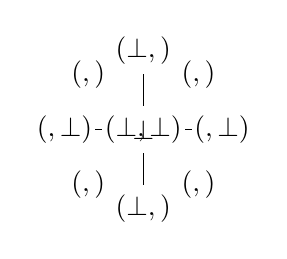
\begin{tikzpicture}

    \begin{scope}
        \myGlobalTransformation{0}{0};
        \node (bottom) at (0,0) {$\bot$};

        \myGlobalTransformation{0}{1};
        \node (botbot) at (0,0) {$(\bot,\bot)$};

        \myGlobalTransformation{0}{3};
        \node (trubot) at (-1,0) {$(\tru,\bot)$};
        \node (bottru) at (0,1)  {$(\bot,\tru)$};
        \node (falbot) at (1,0)  {$(\fal,\bot)$};
        \node (botfal) at (0,-1) {$(\bot,\fal)$};

        \myGlobalTransformation{0}{5};
        \node (trutru) at (-0.7, 0.7) {$(\tru,\tru)$};
        \node (faltru) at ( 0.7, 0.7) {$(\fal,\tru)$};
        \node (falfal) at ( 0.7,-0.7) {$(\fal,\fal)$};
        \node (trufal) at (-0.7,-0.7) {$(\tru,\fal)$};

        \draw (bottom) -- (botbot);

        \draw (botbot) -- (trubot);
        \draw (botbot) -- (bottru);
        \draw (botbot) -- (falbot);
        \draw (botbot) -- (botfal);

        \ddraw{trubot}{trutru};
        \ddraw{bottru}{trutru};
        \ddraw{falbot}{faltru};
        \ddraw{bottru}{faltru};
        \ddraw{trubot}{trufal};
        \ddraw{botfal}{trufal};
        \ddraw{botfal}{falfal};
        \ddraw{falbot}{falfal};

    \end{scope}

\end{tikzpicture}

%\end{document}}
%  \caption{Two partial orders as Hasse Diagrams}
%  \label{fig:pos}
%\end{figure}

\begin{wrapfigure}[25]{r}{0.4\textwidth} %\begin{figure}\begin{figure}[h!]
\begin{center}
\vspace{-30pt}
%\documentclass[10pt]{article}
\newcommand{\myGlobalTransformation}[2]
{
    \pgftransformreset;
    \pgftransformcm{1.6}{0}{0.6}{0.5}{\pgfpoint{#1cm}{#2cm}}
}

\newcommand\tru{\hs{T}}
\newcommand\fal{\hs{F}}

\newcommand\ddraw[2]{
        \draw[-,line width=3pt,draw=white] (#1) -- (#2);
        \draw (#1) -- (#2);
}

%\begin{document}
%\pagestyle{empty}

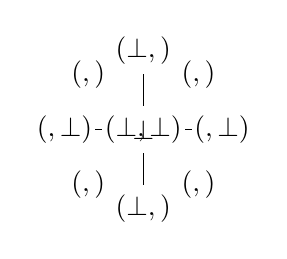
\begin{tikzpicture}

    \begin{scope}
        \myGlobalTransformation{0}{0};
        \node (bottom) at (0,0) {$\bot$};

        \myGlobalTransformation{0}{1};
        \node (botbot) at (0,0) {$(\bot,\bot)$};

        \myGlobalTransformation{0}{3};
        \node (trubot) at (-1,0) {$(\tru,\bot)$};
        \node (bottru) at (0,1)  {$(\bot,\tru)$};
        \node (falbot) at (1,0)  {$(\fal,\bot)$};
        \node (botfal) at (0,-1) {$(\bot,\fal)$};

        \myGlobalTransformation{0}{5};
        \node (trutru) at (-0.7, 0.7) {$(\tru,\tru)$};
        \node (faltru) at ( 0.7, 0.7) {$(\fal,\tru)$};
        \node (falfal) at ( 0.7,-0.7) {$(\fal,\fal)$};
        \node (trufal) at (-0.7,-0.7) {$(\tru,\fal)$};

        \draw (bottom) -- (botbot);

        \draw (botbot) -- (trubot);
        \draw (botbot) -- (bottru);
        \draw (botbot) -- (falbot);
        \draw (botbot) -- (botfal);

        \ddraw{trubot}{trutru};
        \ddraw{bottru}{trutru};
        \ddraw{falbot}{faltru};
        \ddraw{bottru}{faltru};
        \ddraw{trubot}{trufal};
        \ddraw{botfal}{trufal};
        \ddraw{botfal}{falfal};
        \ddraw{falbot}{falfal};

    \end{scope}

\end{tikzpicture}

%\end{document}
\caption{
    \texttt{(Bool,Bool)} partial order.
    \label{fig:boolboolcpo}
}
\end{center}
\end{wrapfigure} %\end{figure}
For tuples and other constructors that take other data types as
parameters, the ordering is:
\begin{equation*}
\hstup{x_0}{y_0} \sqsubseteq_{(a,b)} \hstup{x_1}{y_1} \text{\quad iff \quad}
x_0 \sqsubseteq_a x_1 \text{\w and \w} y_0 \sqsubseteq_b y_1
\end{equation*}

The Hasse Diagram for the \hs{(Bool,Bool)} values can be seen in
Figure \ref{fig:boolboolcpo}. Here \hs{True} is abbreviated for \hs{T}
and similarly for \hs{False}. It is not flat as the one for \hs{Bool};
it can be seen as three dimensional. On the lowest layer the only
value is $\bot$, on the next layer $\hstup{\bot}{\bot}$. Above that
the tuples with one $\bot$, and finally the total values at the
top.

\vspace{55pt}

\subsection{Monotonicity}
 An important property all safe Haskell functions have is that they are
monotone with respect to this ordering.

\paragraph{Definition} A function $f$ is \emph{monotone} iff

\begin{equation*}
\faa{x}{y} \quad x \sqsubseteq y \quad \Rightarrow \quad f(x) \sqsubseteq f(y).
\end{equation*}

This can be understood in many ways. One way to see it is if you have
two inputs to a function, one containing \emph{less} information that
the other, i.e. more bottoms, it is impossible to return \emph{more}
information from the input with less information.

\newpage

One simple example of a consequence of this is the impossibility to
make a function \hs{isBottom :: a -> Bool}, returning \hs{True} if the
argument is bottom, and \hs{False} otherwise:

\note{rewrite with code}
\begin{align*}
& \hs{isBottom} \w :: \hs{a} \rightarrow \hs{Bool} \\
& \hs{isBottom} \w \bot = \hs{True} \\
& \hs{isBottom} \w x \, = \hs{False}, \qquad x \neq \bot
\end{align*}

\noindent
Since $\bot \sqsubseteq x$ for any $x$, then by monotonicity we must
necessarily have
$$\hs{isBottom} \w \bot \sqsubseteq \hs{isBottom} \w x.$$
Take any non-bottom $x$, and this equation gives
$\hs{True} \sqsubseteq \hs{False}$, which is false. Hence
\hs{isBottom} is not monotone.

\subsection{Continuity}
Another domain theoretic property that Haskell functions have is that
they are continuous. This is a property that gives us insight in how
functions behave on infinite input.  To describe this, we need to
consider the partial order of a data type with infinite values. The
prime candidate \hs{data Nat = Zero | Succ Nat} is used and Hasse
Diagram can be seen in Figure \ref{fig:natcpo}.

\begin{figure}[h]
\centering
\usetikzlibrary{positioning,shadows,arrows}

\def\adots{\mathinner{\mkern2mu\raise\hbox{.}
\mkern2mu\raise4\hbox{.}\mkern1mu
\raise8\vbox{\kern7\hbox{.}}\mkern1mu}}


%\begin{tikzpicture}[scale=10]
%
%  \node (bottom)                          {$\bot$};
%  \node (zero)        [above=of bottom]   {$Zero$};
%  \node (suc bot)     [right=of zero]     {$Suc \, \bot$};
%  \node (suc zero)    [above=of suc bot]  {$Suc \, Zero$};
%  \node (suc suc bot) [right=of suc zero] {$Suc \, (Suc \, \bot)$};
%
%  \draw [-] (bottom) -- (zero);
%  \draw [-] (bottom) -- (suc bot);
%  \draw [-] (suc bot) -- (suc zero);
%  \draw [-] (suc bot) -- (suc suc bot);
%
%\end{tikzpicture}
%
\begin{tikzpicture}[grow'=up,sibling distance=2cm]
\node {$\bot$}
    child {
        node {$\hs{Zero}$}
    }
    child {
        node {$\hs{Succ} \, \bot$}
        child {
            node {$\hs{Succ} \, \hs{Zero}$}
        }
        child {
            node {$\hs{Succ} \, (\hs{Succ} \, \bot)$}
            child {
                node {$\hs{Succ} \, (\hs{Succ} \, \hs{Zero})$}
            }
            child {
              node {$ ^{ ^{\adots}}$}
              child [edge from parent/.style={draw=white}] { }
              child {
                node {$\hs{inf}$}
              }
            }
        }
    }

\end{tikzpicture}


\caption{
    The (complete) partial order for \texttt{Nat}, with \hs{inf = Succ inf.}
    \label{fig:natcpo}
}
\end{figure}

At the top we have the infinite value \hs{inf}, defined in Haskell as
\hs{inf = Succ inf}. Here \hs{inf} is the \emph{limit} of an
$\omega$-chain, i.e a chain with the same number of elements as
$\omega$, the natural numbers. The chain is:

\begin{equation*}
\bot \sqsubseteq
\hs{Succ} \, \bot \sqsubseteq
\hs{Succ} \, (\hs{Succ} \, \bot) \sqsubseteq
\hs{Succ} \, (\hs{Succ} \, (\hs{Succ} \, \bot)) \sqsubseteq
\cdots
\end{equation*}

This chain could succinctly be written $\langle \hs{Succ}^n \, \bot
\rangle_{n \in \omega}$.  Here $\hs{Succ}^n$ means $n$ applications of
the \hs{Succ} constructor. The limit is written $\lub{n \in
  \omega}(\hs{Succ}^n \, \bot)$ and is equal to \hs{inf}, where
$\lub{}$ is the least upper bound. All elements in the chain satisfy
the property of being less than or equal to the limit: $\hs{Succ}^n \,
\bot \sqsubseteq \hs{inf}$.

A partial order is a complete partial order iff there is a limit for
every $\omega$ chain. All data types in Haskell are complete partial
orders\footnote{Notice that the data type \hs{data StrictNat = Zero |
    Succ !StrictNat} is flat and therefore complete.}. Now we can
define continuity.

\paragraph{Definition} A function $f$ is \emph{continuous} iff it is
monotone and preserves the $\lub{ }$ of all $\omega$-chains: i.e.
assume any chain $\langle x_n \rangle_{n \in \omega}$, then:

\begin{equation*}
\lub{n \in \omega} \, (f \, x_n) \eq f \, (\lub{n \in \omega} \, x_n)
\end{equation*}

Just as with monotonicity, there are several ways to interpret
this. One way is to say that what a function does on a chain, it must
also do on the chain's limit, as with \hs{map} on increasingly longer
lists. Another is to say that a function cannot produce finite output by
inspecting infinite input: there is no function
\hs{isFinite :: [a] -> Bool} returning \hs{True} on finite lists and
\hs{False} on infinite lists. On the increasing chain
$$ \bot \sqsubseteq x_0 \hs{:} \bot \sqsubseteq x_0 \hs{:} x_1 \hs{:} \bot
\sqsubseteq \cdots$$
the function \hs{isFinite} returns \hs{True} (or $\bot$), but the
limit should return \hs{False}, so this is not a continuous function.

An interesting formulation of Church's Thesis in terms of continuity
is given by Plotkin \cite{domains}:

\begin{center}
\emph{A function is continuous iff it is physically feasible.}
\end{center}

This means that all computable functions are contiuous, and the other
way around. The conclusion for us is that all Haskell functions are
continuous.

\subsection{Unsafe Haskell}
In GHC, you can use \hs{unsafePerformIO} and \hs{catch} from
\hs{Control.Exception} and other tricks to unsafely catch errors
(bottoms). With this machinery it is possible to write a function
\hs{isBottom :: a -> Bool} to catch calls to \hs{undefined}, pattern
match failures, etcetera. In addition, some non-termination some can
also be catched in Haskell because of the \emph{blackhole} run time
object that replaces a \emph{thunk} that is being currently
evaluated. It does not and indeed cannot cover all non terminating
functions because of the undecidability of the Halting problem.

The domain theoretic results remain; one can see $\bot$ as another,
albeit inconveniently inspected, constructor to every data type. All
patterns are exhaustive: every function has an implicit match any
pattern to $\bot$.  Then we add a \emph{true} bottom to the domain
denotes the uncatchable bottoms; undeterminable non termination. With
this setting all Haskell functions are continuous with respect to the
\emph{true} bottoms. But for the rest of this thesis, we shall only
consider pure and safe Haskell functions.

\subsection{Monotonicity as Verification}

Continuity is a concept that is hard to express in first order logic:
it in not able to express countability. We can come close with an
axiomatization of set theory, but we leave that issue and focus on
monotonicity. A way to verify the translation is to add axioms to the
generated theory describing the $\sqsubseteq$ relation, and axioms
that asserts that each function is monotone. An automated theorem
prover could not easily show that it is a satisfiable theory since it
will normally only have infinite models. However, a long run without
any counter model could be seen as a witness for a successful
translation in this respect.


\section{Future Work}

Haskell is a big language, and translating it all in one go is a
daunting task. Therefore, some restrictions were settled to be able to
focus on proving rather than translating.  The goal was to add enough
of the Haskell language to enable to prove interesting properties, but
much of the widely available sugar in Haskell was omitted since it
does not add extra expressibility. This means that list comprehensions
and are not supported but can be added by their respective rewriting
rules. \hs{Type} definitions should be unrolled, so they could be
used in the signature for properties. Type classes is probably the
most interesting thing to add, and is discussed in Section
\ref{sec:typeclasses} in future work.

Another interesting but omitted feature are the built-in types
\hs{Int}, \hs{Integer}, \hs{Double}, \hs{Char}, etc. For \hs{Integer}
appropriate axioms could be added that hold for $\mathbb{Z}$, the
canonical infinite discretely ordered commutative ring.  The other
data types do not enjoy such well behaved properties because of
different bit sizes and overflow and precision errors.

Syntactic features for controlling lazy and strict evaluation namely
irrefutable patterns, \hs{seq} and bang patterns, and richer pattern
matching in form of pattern bindings are discussed below.

\begin{comment}
 It should be
noted that it is already possible to prove a lot of interesting
Haskell properties, it is far from able to prove things about bigger
Haskell projects which usually use a richer part of the language.
\end{comment}

\subsection{Irrefutable Patterns and Pattern Bindings}

Irrefutable patterns can be defined in terms of projections, examples
are \hs{fst}, \hs{snd}, \hs{head}, \hs{fromJust} defined in the
standard library. Each irrefutable pattern is translated to a
constant, and when you use the variables in the pattern, you translate
it to appropriate use of projections. One example is the translation
of the \hs{uncurry} function:

\begin{code}[mathescape]
uncurry f ~(x,y) = f x y        $\Rightarrow$      uncurry f t = f (fst t) (snd t)
\end{code}

\noindent
The irrefutable pattern \verb:~(x,y): is replaced with the new constant
\hs{t}, and in the body of the function, \hs{x} is replaced with the
strict projection \hs{fst t}, and similarly for \hs{y}.

Top level patterns, also called pattern bindings, can
also be written in terms of such projections. The whole pattern
is replaced with a constant, and when the variables from the pattern
are used, you again replace it with projections. This is how it
could look for a simple \hs{fromJust . lookup} implementation:

\begin{code}[mathescape]
unsafeLookup x xs = v           $\Rightarrow$      unsafeLookup x xs = fromJust t
  where Just v = lookup x xs            where t = lookup x xs
\end{code}

The strict projections would not rely on the user having \hs{fst} or
\hs{fromJust} in scope, they can automatically be generated by
inspection of the data type definition.

\subsection{Bang Patterns and \texttt{seq}}

The translations for bang patterns and \hs{seq} are also
straightforward. \hs{seq} defined by bang patterns is:

\begin{code}
seq :: a -> b -> b
seq !x y = y
\end{code}

The axioms for a translation of \hs{seq} needs to ensure that if
\hs{x} evaluates to $\bot$, then \hs{seq x} also evaluates to
$\bot$. The two axioms for this functions are:
\begin{align*}
\rom{1} \qquad & \fa{y}    seq(\bot,y) \eq \bot \\
\rom{2} \qquad & \faa{x}{y} x \neq \bot \rightarrow seq(x,y) \eq y
\end{align*}

Either you implement bang patterns in this fashion, or you do the same
translation as GHC for bang patterns: for each strict variable, you
add a \hs{seq} for that variable for the expression of that pattern,
and you simply add the axioms for \hs{seq} to the theory if the
program uses it or bang patterns. For data types with strictness
fields one proceeds by adding \hs{seq} when constructing elements.

\subsection{Pattern Guards}

Patterns guards is a GHC specific extension to Haskell which allows
arbitrary pattern matching on the result from an expression in a
guard. An example is this elaboration of the \hs{lookup} function from
the \hs{Prelude}, which applies a function to the element, if found:

\begin{code}
transformLookup :: Eq k => k -> [(k,v)] -> (k -> v -> b) -> Maybe b
transformLookup k xs f | Just v <- lookup k xs = Just (f k v)
                       | otherwise             = Nothing
\end{code}

\noindent
If the look up returns \hs{Just}, \hs{v} is already bound and can be
used in the expression of the right hand side. This is very similar to
normal guards, as they are a special case of pattern guards: the guard
\hs{f x | p x} is expressed as \hs{f x | True <- p x}. The current
translation of guards checks if \hs{p x} is \hs{True}, and then
``picks'' this branch, or is $\bot$. This could be done for
constructors, bottoms would need to be added in the guard branches as
is currently done for ordinary patterns.



\chapter{Proof Techniques}

To prove things using this technique, properties are entered in the
Haskell source code. A small prelude called \hs{AutoPrelude} needs to
be imported that gives access to the relevant functions. One example
is the associativity of list concatenation:

\begin{code}
import AutoPrelude

prop_app_assoc :: [a] -> [a] -> [a] -> Prop [a]
prop_app_assoc xs ys zs = xs ++ (ys ++ zs) =:= (xs ++ ys) ++ zs
\end{code}

The infix function \hs{=:=} comes from the import, as well as the type
constructor \hs{Prop}. The type signature cannot be omitted as this is
used for some proof techinques. For induction, you need to see which
kind of induction we will use.

Running the program is simple. Just save the file as for instance
\hs{ListProps.hs} and run

\begin{code}
autospec ListProps.hs
\end{code}

\noindent
and the program will report if it was provable or not, and which
techniques succeeded. Equational properties written like this are also
testable with QuickCheck, so you can run the normal \hs{quickCheck}
function on them, given that there are appropriate \hs{Eq} and
\hs{Arbitrary} instances provided.

The rest of this chapter explains the different proof methods
supported in this tool: definitional equality (Section
\ref{sec:equality}), structural induction (Section
\ref{sec:induction}), fixed point induction (Section
\ref{sec:fixpoint}) and approximation lemma (Section
\ref{sec:approx}).
% Definitional Equality -------------------------------------------------------

\section{Definitional Equality}
\label{sec:equality}

Some properties cannot or need not use induction or some more
sophisticated technique, since they are true by definition. Examples
are properties for fully polymorphic functions such as the definition
of \hs{id} in the SK-calculus, here

\begin{code}
s f g x = f x (g x)
k x y = x
id x = x

prop_skk_id :: Prop (a -> a)
prop_skk_id = s k k =:= id
\end{code}

Then, the generated conjecture is simply

\begin{equation*}
\app{ (\app {\ptr{s}} {\ptr{k}} )
    }{\ptr{k}} = \ptr{id}
\end{equation*}

Another example where this is useful is to prove functor and monad
laws for the environment monad.

\subsection{Extensional Equality and seq}

To prove the previous property we also need to have extensional
equality, postulated with the following axiom

\begin{equation*}
\faa{f}{g} (\fa{x} \app{f}{x} = \app{g}{x}) \rightarrow f = g
\end{equation*}

\noindent
which identifies function pointers and functions composed with $@$.
One problem with extensional equality in Haskell, is that the presence
of \hs{seq} breaks it. \hs{seq} is a built in function with the
following behavior:

\begin{code}[mathescape]
seq :: a -> b -> b
seq $\bot$ y = $\bot$
seq x y = y$, \qquad x \neq
\end{code}

It forces the first argument to weak head normal form and returns the
second. For our purposes, it is only important if the first argument
is $\bot$, then the function also returns this as it is strict in its
first argument. With \hs{seq} it is possibly to distinguish between
these two functions, which otherwise are observationally equal:

\begin{code}[mathescape]
f = $\bot$
g = \x -> $\bot$
\end{code}

Because \hs{seq f ()} evaluates to $\bot$, and \hs{seq g ()} evaluates
to \hs{()}, but on any argument \hs{f} and \hs{g} gets, they both
return $\bot$. Here we also need an extra axiom, which says that
anything applied to $\bot$ is $\bot$:

\begin{equation*}
\fa{x} \app{\bot}{x} = \bot
\end{equation*}

However, \hs{seq} is the only function that can tell such functions
apart, so we will ignore its presence in Haskell.  In the future,
there could be added as a switch \hs{--enable-seq}, which weakens
extensional equality appropriately.

Furthermore, if extensional equality is assumed we also have
the property that \hs{Prop (a -> b)} is equivalent to
\hs{a -> Prop b}, by letting the property have an extra argument that
is applied to the left and right hand side of the equality. This has
two benefits. Firstly, it can trigger other proof methods should \hs{a}
or \hs{b} be concrete types (the former for induction and the latter
for approximation lemma). Secondly, it does not need to use the
extensionality axiom introduced above which introduces extra steps in
the proof search.

\subsection{Future Work: Concrete Concerns}

This only works on non-concrete types because of the way bottoms are
added. One example when this is a problem with is this plausible
definition of boolean or, and the property of right identity:

\begin{code}
False || a = a
True  || _ = True

prop_or_right_identity :: Bool -> Prop Bool
prop_or_right_identity x = x || False =:= x
\end{code}

The translation of \hs{||} makes any element in the domain that is not
the introduced constants $\fn{false}$ or $\fn{true}$ for \hs{Bool}'s
constructors, equal $\bot$. Now consider the translation of the
property:

\begin{equation*}
\fa{x} x \, \fn{||} \, \fn{false} = x
\end{equation*}

Now this is false: take a model with another element $\star$ in the
domain:

$$\star \, \fn{||} \, \fn{false} = \bot$$

The consequence of this is that the proof principle of definitional
equality is only used on abstract types, rather than polymorphic, as
they cannot be strict. Do not fear: the property above is trivially
proved by induction. For the \hs{Bool} type and other non recursive
data types, induction degenerate into mere case enumeration.




% Structual Induction ---------------------------------------------------------

\section{Structural induction}

\subsection{Induction}

Some background of induction and how it is present in well-known
theories like PA, ZFC, MLTT and CoC.

PA which only concerns natural numbers has a small vocabulary
consisting only of the constant $0$, the unary successor function $s$,
and binary plus and multiplication.
Here the induction schema from looks like this:

\note{One could also be explicit about the free variables in $P$}
\begin{mathpar}
  \inferrule*
     {
       \overbrace{P(0)}^{\mathrm{base}}
       \\
       \overbrace{
           \fa{x}
                 \underbrace{P(x)}_{\mathrm{hypothesis}}
              \rightarrow
                 \underbrace{P(s(x))}_{\mathrm{conclusion}}
       }^{\mathrm{step}}
     }
     { \fa{x} P(x) }
\end{mathpar}

This is a axioms schema since it is not possible to quantify over the
predicate $P$ in FOL. Rather, it is a infinite set of axioms, one for
each (well-formed) formula instantiated in place for $P$. Generally,
ATPs do not instantiate schemas themselves but it has to be done
manually, with an appropriate formula for $P$.

Any non-recursive, or more importantly recursive data type gives rise
to induction schemata.

\footnote{Haskell's natural numbers are of course also cluttered with
  elements that are not natural numbers, such as $\bot$, but also the
  infinite ``natural number'' defined by \hs{infinite = Succ infinite}}
, defined the usual way in Haskell by \hs{data Nat = Zero | Succ Nat}
yields this induction axiom schema:

\begin{mathpar}
  \inferrule*
     {
       P(\fn{Zero})
       \\
       \fa{x} P(x) \rightarrow P(\fn{Succ}(x))
     }
     { \fa{x} P(x) }
\end{mathpar}


% Fixpoint Induction ----------------------------------------------------------

\section{Fixed point induction}
\label{sec:fixpoint}

Induction is applicable when arguments are of a concrete type, such as
lists or natural numbers. There are also properties where all
arguments are of abstract types. The canonical example is the
map-iterate property:

\begin{equation*}
\faa{(f : a \rightarrow a)}{(x : a)} \hs{map} \w f \w (\hs{iterate} \w f \w x) \eq
           \hs{iterate} \w f \w (f \w x)
\end{equation*}

Here $f$ is an abstract function $a \rightarrow a$, and $x$ is
something of type $a$. This example is further investigated in Section
\ref{sec:mapiter} below, but it is already clear that we cannot proceed to
prove this with structural induction.

Enter fixed point induction. It allows a way of performing induction
on the recursive structure of the program. In short, if the property
regards a function $f$, the hypothesis is that the property holds for all
the recursive calls in the definiton of $f$, and the goal is to prove
that it holds for $f$.

\begin{comment}
It
is an early example of a technique from domain theory, attributed to
Scott and de Bakker,
\note{Citation needed: there is a book called
  Mathematical Theory of Program Correctness by Jaco de Bakker that
  could be appropriate if found}
and sometimes called Scott induction
or computational induction.  \cite{domains}
\end{comment}

The least fixed point for a function can be found in Haskell with the
function \hs{fix}, which can simply be defined as:

\begin{code}
fix :: (a -> a) -> a
fix f = f (fix f)
\end{code}

This function solves the equation $x = f \w x$, since substituting $x$
for $\hs{fix} \w x$: the left side evaluates to $f \w (\hs{fix} \w f)$
in one step, which is then equal to the right side. This is the origin
of the name of the combinator \hs{fix}: this is a fixed point of the
equation.  Any self-recursive function can be rewritten in terms of
\hs{fix}. Recall the \hs{Prelude} function \hs{repeat}, which makes an
infinite list of the same element \hs{repeat x = x : repeat}. Its
transformation to \hs{fix}-style is this:

\begin{code}
repeat x = fix r
  where r i = x : i
\end{code}

Computing \hs{repeat x}, we get the following unfolds:
\begin{equation*}
  \hs{repeat x}
= \hs{fix r}
= \hs{x:fix r}
= \hs{x:x:fix r}
= \hs{x:x:x:fix r}
  \cdots
\end{equation*}
So \hs{fix (x:)} is the infinite list of \hs{x}. The translation of a
self-recursive function to be defined in terms of \hs{fix} is
mechanical. Assume $f$ is defined with arguments $\overline{x}$ and
has a body $e$ that uses both itself and its arguments, let us write
this as $e(f,\overline{x})$. Then the translation is this:

\begin{equation*}
f \w \overline{x} \eq e(f,\overline{x})
\w \Leftrightarrow \w
f \eq \hs{fix} \w (\lambda \w f' \w \overline{x} \w \rightarrow \w e(f',\overline{x}))
\end{equation*}

Another more domain theoretic approach is to say that
$\hs{fix} \w f \eq \lub{n}(f^n \bot)$, where $f^n \bot$ is $n$ applications of $f$:
\begin{equation*}
f^n \bot \eq \underbrace{f (f (\cdots (f}_{n \w \mathrm{copies \w of} \w f}} \bot) \cdots))
\end{equation*}
This corresponds to a potentially infinite, countable unrolling of $f$.
It is easy to verify that $\langle f^n \bot\rangle_{n\in\omega}$ is a
$\sqsubseteq$-chain by induction on $n$, and that this is the least
pre-fixed point of $f$ is also showed by induction: Assume there
is another pre-fixed point $\theta$, thus satisfying
$\theta \eq f \w \theta$. The base case is
$\bot \eq f^0 \bot \sqsubseteq \theta$, trivially satisified since
$\bot$ is the least element. For the step case, assume that
$f^n \bot \sqsubseteq \theta$, and we get the conclusion
$f^{n+1} \bot = f (f^n \bot) \sqsubseteq f \w \theta = \theta$ as desired.
Fixpoint induction proves properties about a function written in terms
of \hs{fix}, and its inference rule is this:

\begin{mathpar}
  \inferrule*
     {
       P(\bot)
       \\
       P(x) \rightarrow P(f \w x)
       \\
       P \w \mathrm{admissible}
     }
     { P(\fn{fix} f) }
\end{mathpar}


Here it is important that $P$ is \emph{admissible} , meaning that for
all $\sqsubseteq$-chains of length $\omega$, if the property holds for
all elements in the chain it must necessary hold for its limit, futher
described in Section \ref{sec:admissible}, where a proof is given that
the properties we are interested in, universally quantified equalities
of continuous functions, are admissible predicates.

An interesting property of fixed point induction is that it does not
care about types: indeed, it works in an untyped setting. In addition,
it can exploit strange recursive structures of the function. A caveat
is that it can only prove properties that must hold for infinite and
partial values.

The proof that fixed point induction relies on the fact that
$\lub{n}(f^n \w \bot) \eq \hs{fix} \, f$, where $f^n$ is $n$
self-applications of $f$. This is true since \hs{fix} is defined as
$f$ self-applied to it self. Apart from this, the proof only uses
induction over natural numbers and that $f^0 \w \bot \eq \bot$, and
it is of course important that $P$ is admissible. See proof below:

\begin{align*}
P(\bot) & \wedge \fa{x} P(x) \rightarrow P(f x) \\
\desclra{$f^0 \w \bot \eq \bot$} \\
P(f^0 \w \bot) & \wedge \fa{x} P(x) \rightarrow P(f x) \\
\descra{quantifying} \\
P(f^0 \w \bot) & \wedge \fa{n} P(f^n \w \bot) \rightarrow P(f^{n+1} \w \bot) \\
\desclra{induction} \\
\fa{n} & P(f^n \w \bot) \\
\desclra{\textit{P} \w admissible} \\
& P(\lub{n}(f^n \w \bot)) \\
\desclra{definition \w of \w \hs{fix}} \\
& P(\hs{fix} \w f) \\
\end{align*}

One reason to introduce fixed point induction is to avoid the natural
numbers in $\fa{n} P(f^n \bot)$  to prove $P(\hs{fix} \w f)$.

\subsection{Example: map-iterate}
\label{sec:mapiter}

For properties that do not have any arguments with a concrete type,
structural induction is not applicable. The Haskell function
\hs{iterate} is a that makes an infinite list from a seed, by repeated
application of a function, i.e \hs{iterate f x} is the list
 \hs{x:f x:f (f x):}$\cdots$. It is related to Haskell function
 \hs{map} in the map-iterate property, stated as follows:

\begin{equation*}
\faa{f}{x} \hs{map} \w f \w (\hs{iterate} \w f \w x) \eq
           \hs{iterate} \w f \w (f \w x)
\end{equation*}

\noindent
With their standard definitions given in \ref{code:mapiterate} below.

\begin{figure}[h!]
\centering
\begin{minipage}[b]{6cm}
\begin{code}
map :: (a -> b) -> [a] -> [b]
map f (x:xs) = f x : map f xs
map f [] = []
\end{code}
\end{minipage}
\hspace{10pt}
\begin{minipage}[b]{6cm}
\begin{code}[mathescape]
iterate :: (a -> a) -> a -> [a]
iterate f x = x : iterate f (f x)
$\newline$
\end{code}
\end{minipage}
\caption{Definition of \texttt{map} and \texttt{iterate}
\label{code:mapiterate}
}
\end{figure}

The behavior of \hs{map} is to apply a function to every element of a
list. We see that we cannot use structural induction here, since both
$f$ and $x$ are abstract, but this can be proved by fixpoint induction
on \hs{iterate}. First, we rewrite this function in terms of \hs{fix}:

\begin{code}
iterate = fix iter
iter i f x = x : i f (f x)
\end{code}

The predicate $P$ from fixpoint induction is $P(g) \w \Leftrightarrow
\w \faa{f}{x} \hs{map} \w f \w (g \w f \w x) \eq g \w f \w (f \w x) $. If we
prove the base case and step case we can then conclude
$P(\hs{fix iter})$, and that is by definition $P(\hs{iterate})$.

The base case is $P(\bot)$. Since \hs{map} is strict in its second
argument, it is both the left side and right side evaluate to $\bot$.
The for the step case we have to show
$P(\hs{i}) \rightarrow P(\hs{iter i})$. We start from the induction
hypothesis and work towards the goal as follows:

\begin{align*}
\w \faa{f}{x} \hs{map} \w f \w (\hs{i} \w f \w x) & \eq \hs{i} \w f \w (f \w x) \\
\descra{generalizing $x$ to $f \w x$} \\
\w \faa{f}{x} \hs{map} \w f \w (\hs{i} \w f \w (f \w x)) & \eq \hs{i} \w f \w (f \w (f \w x)) \\
\descra{substitutivity} \\
\w \faa{f}{x} f \w x \hs{:} \hs{map} \w f \w (\hs{i} \w f \w (f \w x)) & \eq f \w x \hs{:} \hs{i} \w f \w (f \w (f \w x)) \\
\desclra{\defof{\texttt{map}}} \\
\w \faa{f}{x} \hs{map} \w f \w (x \hs{:} \hs{i} \w f \w (f \w x)) & \eq f \w x \hs{:} \hs{i} \w f \w (f \w (f \w x)) \\
\desclra{\defof{\texttt{iter}}} \\
\w \faa{f}{x} \hs{map} \w f \w (\hs{iter} \w \hs{i} \w f \w x) & \eq \hs{iter} \w \hs{i} \w f \w (f \w x) \\
\end{align*}

As discussed earlier, the $P$ used is admissible since it is an
universally quantified equality. Hence, fixpoint induction gives us the
\hs{map}-\hs{iterate} property.


\begin{comment}
To illustrate why it is important that the property $P$ is admissible,
we shall consider an example
consider the predicate P to be “is not infinite”, and then you can
prove for a lot of functions that they return finite objects. For
instance, define this function:

CHANGE THIS

  Instead do the finite list predicate, and use $\neq
  \hs{False}$. This then servers for an example why inequality
  predicates are not admissible!

\begin{code}
listrec :: ([a] -> [a]) -> [a] -> [a]
listrec i [] = []
listrec i (x:xs) = x : i xs
\end{code}

Then define
$P(f) \Leftrightarrow \fa{x} ``f(x) \w \mathrm{is \w not \w infinite}"$,
and proceed to prove $P(\hs{fix listrec})$ by fixed point induction. The
base case $P(\bot)$ succeeds, since $\bot$ is not infinite, and if we
assume $P(\hs{i})$, we have no problem proving $P(\hs{listrec i})$.
Hence $P(\hs{fix listrec})$, and since \hs{fix listrec} is essentially
a linear identity function on lists, we have ``proved'' that all lists
are finite (but possibly partial).

The error is as promised that $P$ is not admissible: for the sequence
\begin{equation*}
\bot \sqsubseteq
\hs{0:}\bot \sqsubseteq
\hs{0:1:}\bot \sqsubseteq
\hs{0:1:2:}\bot \sqsubseteq
\cdots
\end{equation*}
$P$ holds for all elements but $P$ does not hold for its limit \hs{[0..]}.

\end{comment}

\begin{comment}
\subsection{Mutually Recursive Functions}

You can also mechanically transform mutually recursive functions to be
defined in terms of \hs{fix}. The functions \hs{even} and \hs{odd}
defined below, which determines if a \hs{Nat} is even, and odd,
respectively, are straightforwardly written by mutual recursion:

\begin{code}
even :: Nat -> Bool           odd :: Nat -> Bool
even Z     = True             odd Z     = False
even (S x) = odd x            odd (S x) = even x
\end{code}

To write these functions in terms of fix, as an additional argument,
the take a tuple of ``non-recursive'' copies of themselves.

\begin{code}
evenToFix :: (Nat -> Bool,Nat -> Bool) -> Nat -> Bool
evenToFix (evenUnFix,oddUnFix) Z     = True
evenToFix (evenUnFix,oddUnFix) (S x) = oddUnFix x

oddToFix :: (Nat -> Bool,Nat -> Bool) -> Nat -> Bool
oddToFix (evenUnFix,oddUnFix) Z     = True
oddToFix (evenUnFix,oddUnFix) (S x) = evenUnFix x
\end{code}

Here the prefix \hs{ToFix} means that it is a function subject to be
\hs{fix}-ed, and \hs{UnFix} means that it is the ``non-recursive''
function. The functions above can now be \hs{fix}-ed by giving the
tuple as an argument to both of them:

\begin{code}
even',odd' :: Nat -> Bool
(even',odd') = fix (\t -> (evenToFix t,oddToFix t))
\end{code}

This encoding makes \hs{even'} denotationally equal to \hs{even} and
the same relation hols for \hs{odd'} and \hs{odd}.
\end{comment}

\subsection{Simplification}

The mechanical translations introduced above for self-recursive
functions and mutually recursive functions makes a new function with
an additional argument, the ``non-recursive'' version of itself. By
the translation to FOL that is used, this would introduce a new
argument as a ``function pointer'' and introduce uses of $\appfn$,
which gives unnecessary overhead to the automated theorem
provers.

This is another approach. It avoids introducing these function
pointers and the additional argument to every function. Given a
function $f$ with arguments $\overline{x}$ defined as this:

\begin{equation*}
f \, \overline{x} = e(\overline{x},f)
\end{equation*}

Two new constants are introduced, $\tofix{f}$ and $\unfix{f}$
and this definition:

\begin{equation*}
\tofix{f} \, \overline{x} = e(\overline{x},\unfix{f})
\end{equation*}

\noindent
The empty circle $\unfix{}$ describes that this function is empty
(lacks implementation,) and the filled circle $\tofix{}$ means that
this function has an implementation.

Now we can get a simplified fixpoint schema:

\begin{mathpar}
  \inferrule*
     {
       P(\bot)
       \\
       P(\unfix{f}) \rightarrow P(\tofix{f})
       \\
       P \, \mathrm{admissible}
     }
     { P(f) }
\end{mathpar}

\noindent
The empty $\unfix{f}$ does not have any implementation. But it has
something much better, namely the induction hypothesis. The induction
conclusion is to prove the property for $\tofix{f}$, where the
recursive call to $f$ is replaced with $\unfix{f}$. We do this
simplification since it is better suited for the theorem provers.

\newpage
This also works for several functions at the same time, possibly
mutually recursive:

\begin{mathpar}
  \inferrule*
     {
       P(\bot,\bot)
       \\
       P(\unfix{f},\unfix{g}) \rightarrow P(\tofix{f},\tofix{g})
       \\
       P \, \mathrm{admissible}
     }
     { P(f,g) }
\end{mathpar}

This translation needs to be carried out with some care, since for $f
\, \overline{x} = e(\overline{x},f)$, it is also possible that $f$ is
called in bodies of other functions. These are of two kinds: either
this function is also called from $f$, making it recursive, or another
function which is not called from $f$, but makes use of $f$
anyway. The first example, with a recursive call, the body needs to be
edited so $f$ becomes translated (to $\bot$, $\unfix{f}$ or
$\tofix{f}$), and the second case should use the original $f$. The
transitive clousure of the call graph is calculated, and every
appropriate calls of $f$ are replaced.

\subsection{Erroneous Use of Fixed Point Induction}

The importance that the predicate $P$ is admissible is illustrated in
this example. The function \hs{finite} below returns \hs{True} on
finite lists and $\bot$ on partial lists.

\begin{code}
finite :: [a] -> Bool
finite []     = True
finite (x:xs) = finite xs
\end{code}

Is it possible to use \hs{finite} to prove that \emph{all} lists in
Haskell are either finite or partial? Let the predicate be
$P(f) \Leftrightarrow \fa{xs} f \w xs \neq \hs{False}$, and proceed by fixed
point induction. This is the proof plan with the predicate inlined:

\begin{mathpar}
  \inferrule*
     {
       \fa{xs} \bot \w xs \neq \hs{False}
       \\
       \fa{xs}             \unfix{\hs{finite}} \w xs \neq \hs{False}
               \rightarrow \tofix{\hs{finite}} \w xs \neq \hs{False}
     }
     { \fa{xs} \hs{finite} \w xs \neq \hs{False} }
\end{mathpar}

\noindent
The base case is trivial, as anything applied to bottom is $\bot$ and
$\bot \neq \hs{False}$. The step case also succeeds; trivially if $xs$
is the empty list, by the hypothesis if $xs$ is non-empty, and if $xs$
is bottom for similar reasons as in the base case.

The error is as promised that $P$ is not admissible. See the
$\sqsubseteq$-chain below:
\begin{equation*}
\bot \sqsubseteq
\hs{0:}\bot \sqsubseteq
\hs{0:1:}\bot \sqsubseteq
\hs{0:1:2:}\bot \sqsubseteq
\cdots
\end{equation*}
$P$ holds for all elements in the chain, but $P$ does not hold for its
limit \hs{[0..]}. This example also serves as a proof that inequality
in general is not admissible.


\subsection{Candidate Selection}

Faced with the following property saying that if you drop $n$ elements
from a list the length of this is the same as the length of the
original list minus $n$, which functions should one do fixed point
induction on?

\begin{verbatim}
prop_length_drop :: [a] -> Nat -> Prop Nat
prop_length_drop xs n = length (drop n xs) =:= length xs - n
\end{verbatim}

The answer here is to do fixed point induction on \hs{drop}, and on
\hs{-}. So far no better way to tackle this is used than to try fixed
point induction on all subsets of recursive functions mentioned in the
property.

\subsection{Future Work}

Just as with structural induction, it is also possible to use fixed
point in more than one ``depth'', giving for instance this inference
rule:

\begin{mathpar}
  \inferrule*
     {
       P(\bot)
       \\
       P(f \w \bot)
       \\
       P(x) \wedge P(f \w x) \rightarrow P(f \w (f \w x))
       \\
       P \w \mathrm{admissible}
     }
     { P(\fn{fix} f) }
\end{mathpar}

It is also possible to use such an encoding as in ``Automated depth''
in Section \ref{sec:futind} to let the theorem prover determine the
depth. As an example, the map-iterate property impossible to show with
\hs{map} redefined to \hs{doublemap}, defined below, with ordinary one
depth fixed point induction.

\begin{verbatim}
doublemap :: (a -> b) -> [a] -> [b]
doublemap f []       = []
doublemap f [x]      = [f x]
doublemap f (x:y:zs) = f x : f y : doublemap f zs
\end{verbatim}

\noindent
While \hs{doublemap} is behaviorally equivalent to \hs{map} on total
lists, it makes the induction hypothesis in fixed point induction too
weak.


An issue with the candidate selection is that is some selections are
quite stupid, for instance doing fixating functions on only one side
of the equality. A heuristic to find good candidates would be beneficial.

% Approximation Lemma ---------------------------------------------------------

\section{Approximation Lemma}

The approximation lemma must be considered a standard technique for
proving properties about corecursive programs. Just like fixed point
induction it can be used with functions that are produce infinite
values, like \hs{repeat} and \hs{iterate}, out of abstract values
making structural induction impossible \cite{corecursive}.  The
approximataion lemma supersedes the classical take lemma
\cite{introfp} by being easier to apply and generalize: unlike the
take lemma, it can be applied to equalities of any polynomial
data type \cite{genapprox}. The definitions of \hs{take} and
\hs{approx}: % for lists can be viewed in figure \ref{fig:takeapprox}.

%% This is weird!

%\floatstyle{ruled}
%\newfloat{program}{thp}{lop}
%\floatname{program}{Program}

\note{how to put/float source code side by side?}
%\begin{program}
\begin{verbatim}
take :: Nat -> [a] -> [a]             approx :: Nat -> [a] -> [a]
take Zero    _      = []              approx (Suc n) []     = []
take (Suc n) []     = []              approx (Suc n) (x:xs) = x : approx n xs
take (Suc n) (x:xs) = x : take n xs
\end{verbatim}
%\caption{Definition of \hs{take} and \hs{approx} on lists, with Peano-\hs{Nat}s.}
%\label{fig:takeapprox}
%\end{program}
\note{write this as Haskell code? (those \hs{Nat} are actually $\mathbb{N}$)}

Whereas \hs{take} approximates a list and ends it with \hs{[]},
\hs{approx} ends it with $\bot$ since the \hs{Zero} case is
omitted. The idea of these techniques is then to show that show that
two lists are equal by showing that their prefix or approximation
coincides for all natural numbers. The approximation lemma is given thusly

\begin{equation}
\label{eq:approxeq}
xs \, = \, ys \quad \Leftrightarrow \quad \fa{n \in \mathbb{N}} \hs{approx} \, n \, xs = \hs{approx} \, n \, ys
\end{equation}

Equation \ref{eq:approxeq} quantifies over the \emph{true} natural
numbers, rather than the \emph{polluted} Haskell naturals. Showing an
equality then amounts to a proof by induction over natural numbers,
and the base case for $0$ is always true by reflexivity, as the
approximation is $\bot$.
The right to left implication is (trivially) true by substitution, and
the other direction hinges on the lemma that better and better
approximations form a chain with limit \hs{id}, as illustrated in
Equation \ref{eq:approxchain}.

\begin{equation}
\label{eq:approxchain}
\hs{approx} \, 0 \,
   \sqsubseteq \,
\hs{approx} \, 1 \,
   \sqsubseteq \,
\cdots
   \sqsubseteq \,
\hs{approx} \, n \,
   \sqsubseteq \,
\hs{approx} \, (\hs{Suc} \, n) \,
   \sqsubseteq \,
\cdots
   \sqsubseteq \,
\hs{id}
\end{equation}

The inclusions in \ref{eq:approxchain} are easily given by induction
on natural numbers and the limit by structural induction on lists.
For other polynomial data types, this lemma is established by
the structural induction induced on that data type.
The desired implication is then readily deduced:

\newcommand{\xsys}[2]{#1 \, xs \, #2 & = #1 \, ys #2}
\newcommand{\desca}[1]{  & \hspace{44.5mm}                              \{ \mathrm{#1} \}}
\newcommand{\descra}[1]{ & \hspace{35mm} \Rightarrow     \hspace{4mm} \{ \mathrm{#1} \}}
\newcommand{\descla}[1]{ & \hspace{35mm} \Leftarrow      \hspace{4mm} \{ \mathrm{#1} \}}
\newcommand{\desclra}[1]{& \hspace{35mm} \Leftrightarrow \hspace{4mm} \{ \mathrm{#1} \}}
\begin{align*}
\xsys{\fa{n} \hs{approx} \, n}{}            \\
\descra{limits}                             \\
\xsys{\lub{n} \, (\hs{approx} \, n}{)}      \\
\desclra{continuity \, of \, application}   \\
\xsys{\lub{n} \, (\hs{approx} \, n)}{}      \\
\desclra{Equation \, \ref{eq:approxchain}} \\
\xsys{\hs{id}}{}                            \\
\desclra{definition \, of \, \hs{id}}       \\
\xsys{}{}                                   \\
\end{align*}

\subsection{Example: Mirroring an Expression}

Consider these definitions of a modest but prototypical expression
data type, and its mirroring function:

\begin{verbatim}
data Expr = Add Expr Expr | Value Nat

mirror :: Expr -> Expr
mirror (Add e1 e2) = Add (mirror e2) (mirror e1)
mirror (Value n)   = Value n

prop_mirror_involutive :: Expr -> Prop Expr
prop_mirror_involutive e = e =:= mirror (mirror e)
\end{verbatim}

Two things to notice here is that the type \hs{Expr} does not have a
nullary constructor. Then the \hs{take} lemma would not be usable as
there is no such function over these expressions: the list version
returns the empty list \hs{[]} for the zero case, but there is no such
alternative for \hs{Expr} above. It is important that the limit of
approximations is the identity, and we cannot get this property when
trying to generalise the take lemma.

Furthermore, fixed point induction fails on this property: choosing
either or both occurrences of \hs{mirror} on the right side is
constant bottom for the base case, and the left side is the identity.


We shall now proceed to prove that \hs{mirror} is involutive by the
approximation lemma. The approximation function for \hs{Expr} is
automatically generated, by approximating each self-recursive
constructor, and hence \hs{Value}'s \hs{Nat} is not further approximated:

\begin{verbatim}
approx :: Nat -> Expr -> Expr
approx (Suc n) (Add e1 e2) = Add (approx n e1) (approx n e2)
approx (Suc n) (Value n)   = Value n
\end{verbatim}

\note{Use $\bot$ or bottom in this text?}
Indeed, we also get a third case for $\bot$ which states that the
approximation of $\bot$ is, quite unsurprisingly, $\bot$.
As always in proofs by approximation lemma, we proceed by induction
over natural numbers, and the base case is always trivial: true by
reflexivity as both sides are $\bot$. The step case - which indeed is
the only proof obligation in any proof of this kind - is to prove
this:

\begin{equation*}
\fa{e}  approx \, (\hs{Suc} \, n) \, e = approx \, (\hs{Suc} \, n) \, (mirror \, (mirror \, e))
\end{equation*}

An important property of the induction hypothesis is the universal
quantification of the expression $e$, unlike the fixed natural number
$n$:

\begin{equation*}
\fa{e}  approx \, n \, e = approx \, n \, (mirror \, (mirror \, e))
\end{equation*}

The proof is by case exhaustion. The case for \hs{Value} and $\bot$
are trivial: \hs{mirror} is strict in its first argument, and
mirroring \hs{Value} twice is the identity, so these cases are both
true by reflexivity. The \hs{Add} case is ever so slightly more
elaborate, and with names shortened to \hs{app} and \hs{mir} the
reasoning is as follows:

\note{$(\hs{Suc} \, n)$ or $(n + 1)$?}
\newcommand{\Adds}[2]{\hs{Add} \, #1 e_1 #2 \, #1 e_2 #2}
\newcommand{\Approxn}[0]{\hs{app} \, n \,}
\newcommand{\ApproxSucn}[0]{\hs{app} \, (\hs{Suc} \, n) \,}
\newcommand{\mirmir}[0]{\hs{mir} \, (\hs{mir} \, }
\begin{align*}
\faa{e_1}{e_2}&  \ApproxSucn (\Adds{}{})  = \ApproxSucn (\mirmir \Adds{}{} ))                                                                   \\
                                                                                 \desclra{\defof{\hs{mirror}}}                                   \\
\faa{e_1}{e_2}&  \ApproxSucn (\Adds{}{})  = \ApproxSucn (\Adds{(\mirmir}{))})                                                                    \\
                                                                                \desclra{\defof{\hs{approx}}}                                    \\
\faa{e_1}{e_2}&  \Adds{(\Approxn}{)}      = \Adds{(\Approxn(\mirmir}{)))}                                                                        \\
                                                                                \desclra{induction \, hypothesis \, twice \, (e_1 \, and \, e_2)} \\
\faa{e_1}{e_2}&  \Adds{(\Approxn}{)}      = \Adds{(\Approxn}{)}                                                                                  \\
                                                                                \desca{reflexivity}                                              \\
\end{align*}

\subsection{Approximation Lemma is Fixpoint Induction}

This technique is already simple and widely applicable, however it can
further be simplified. Implementing it in this form relies on the
auxiliary structure of Peano natural numbers which also needs to be
added to the theory. This can be removed by the observation that is
\note{What is a better name for these functions than \hs{id}?}
expressed as fixed point induction over a recursive form of \hs{id}.

\begin{verbatim}
id :: [a] -> [a]              id :: Expr -> Expr
id []     = []                id (Add e1 e2) = Add (id e1) (id e2)
id (x:xs) = x : id xs         id (Value n)   = Value n
\end{verbatim}

Each \hs{id} function constructed in this way is indeed an identity
function, equivalent to the implementation \hs{id x = x} if we
disregard time and space complexity. Now, to prove

\begin{equation*}
e_1 \, = \, e_2
\end{equation*}

we simply use fixed point induction to prove

\begin{equation*}
\hs{id} \, e_1 \, = \, \hs{id} \, e_2
\end{equation*}

where \hs{id} is a such a specialized recursive identity function over
the data type of the equality. With the same translation of recursive
functions as in the fixed point section, the axioms for \hs{id} for, say
lists becomes:

\begin{align*}
            & \tofix{id}(\hs{[]}) \,   = \, \hs{[]}                                                           \\
\faa{x}{xs} & \tofix{id}(x\hs{:}xs) \, = x\hs{:}\unfix{id}(xs)                                                \\
\fa{xs}     & \tofix{id}(xs)           = \bot  \leftarrow    xs \neq [] \wedge xs \neq head(xs)\hs{:}tail(xs) \\
\end{align*}

The step case in induction $P(\unfix{id}) \rightarrow P(\tofix{id})$
is then exactly the same strength as the approximation lemma with
natural numbers.

\subsection{Implementation} The implementation of approximation lemma
was the simplest to implement, after definitional equality. First,
from the type signature from the property, such a recursive identity
function as above is generated for the data type of the equality. Then
the lemma $P(\unfix{id})$ is added to the theory, with $P$
instantiated to the universally quantified equality, and the
conjecture is $P(\tofix{id})$. The base case need not be proven,
$P(\bot)$ is always true since it evaluates to $\bot=\bot$.

\subsection{Future Work: Total Approximation Lemma}

It is also possible to adjust the approximation lemma to prove
properties that are true for total and potentially infinite objects,
but false for objects with partial values. One such property is the
idempotence of \hs{nub}. Here is a version of \hs{nub} on booleans,
and the said property about it:

\begin{verbatim}
nub :: [Bool] -> [Bool]
nub (True :True :xs) = nub (True:xs)
nub (False:False:xs) = nub (False:xs)
nub (x:xs)           = x:nub xs
nub _                = []

prop_nub_idem :: [Bool] -> Prop [Bool]
prop_nub_idem xs = nub (nub xs) =:= nub xs
\end{verbatim}

Consider the list \hs{True:False:}$\bot$. One application of \hs{nub}
gives \hs{True:}$\bot$, and two gives $\bot$ immediately. In spite of
this, the property is a truism for finite as well as infinite lists,
provided that there are not bottoms.

The way to enable the approximation lemma to prove such properties is
to add predicates of totality, and add axioms like the following to
the theory:

\note{How to make $Total$ look like one word? The kerning for $T$ in
  $Total$ looks incorrect}
\begin{align*}
            & \neg \, Total(\bot) \\
            & Total(\hs{[]}) \\
\faa{x}{xs} & Total(x) \wedge Total(xs) \rightarrow Total(x\hs{:}xs) \\
\fa{xs}     & Total(xs) \rightarrow Total(\hs{nub} \, xs) \\
\end{align*}

To use fixed point induction \hs{Total} needs to be an admissible
predicate. But this is indeed so, for each model with infinite lists,
we have that all such lists are total.  However, that a total argument
to \hs{nub} yields a total value also needs to be proven. Furthermore,
the totality property for the cons case of lists is debatable: should
the consed element also be total?

The proof obligation is then:

\begin{mathpar}
  \inferrule*
     {
        \fa{xs} Total(xs) \Rightarrow \unfix{id}(\hs{nub} (\hs{nub} \, xs)) = \unfix{id}(\hs{nub} \, xs)
     }
     {
        \fa{xs} Total(xs) \Rightarrow \tofix{id}(\hs{nub} (\hs{nub} \, xs)) = \tofix{id}(\hs{nub} \, xs)
     }
\end{mathpar}

It seems like you have to add
$Total(x) \rightarrow Total(\tofix{id}(x))$ and
$Total(x) \rightarrow Total(\unfix{id}(x))$ to the theory, too.

\subsection{Uncategorized / old}

After fixed point induction since it is an easy consequence of fixed
point induction, and how we removed the auxiliary structure of natural
numbers. This makes it equivalent to fixed point induction of id on
both sides (or does it?)

Approximation lemma is a generalization of the take lemma, and its
first form is used for properties about infinite and partial lists,
but it is easily generalized to other recursive data types.
In particular, all polynomial data types — for example, any
sum-of-products data type — can be defined in this way.
This result generalizes
to mutually recursive, parameterised, exponential and nested datatypes, but
for simplicity we only consider polynomial datatypes in this article.
\cite{genapprox}

How to use approximation lemma on exponential, mutually recursive and
nested data types? This would be nice.

%% Results --------------------------------------------------------------------

\chapter{Results and Discussion}
\label{ch:results}

This chapter describes the test suite used in this project. A large
test with five theorem provers was carried out on this test suite, and
this section describes the setup and results.

\section{Test Suite}

To carry out a throughout testing of the system a large test suite was
developed and collected from other sources.  It consists of over 25
Haskell source files, and includes over 500 equality properties.  The
files of can be divided into groups with different aims of complexity,
suitable proving methods and different aspects of Haskell. All files
of the test suite are briefly described in Table \ref{tbl:testsuite},
and available in the project's repository\footnote{See the
  \hs{testsuite} directory in \url{http://github.com/danr/hip/}}, but
some parts and design decisions are highlighted in the rest of this
section.

\begin{table}[p]
\centering
\begin{tabular}{>{\small}l | >{\small}l | >{\small}p{6cm} }
Group              & File                   & Description \\
\hline
Fundamental        & $\ts{Bool                  }$ & Simple properties about and, or and not \\
                   & $\ts{Expr                  }$ & Expressions with mirror, size and eval \\
                   & $\ts{Functions             }$ & Function composition, currying \\
                   & $\ts{Integers              }$ & Integers as a disjoint union of Nats \\
                   & $\ts{Reverse               }$ & Reverse with and without accumulator \\
                   & $\ts{Queues                }$ & Queues with $O(1)$ pop and enqueue \\
Infinite values    & $\ts{Infinite              }$ & Infinite list and tree properties \\
                   & $\ts{Sequences             }$ & Infinite sequences \\
                   & $\ts{Streams               }$ & Streams from \citep{streams} \\
Miscellaneous      & $\ts{PatternMatching       }$ & \hs{||} and \hs{mirror} in different ways \\
                   & $\ts{Fix                   }$ & Even and odd defined using \hs{fix} \\
                   & $\ts{Tricky                }$ & Properties that hold for total infinite lists \\
Monads             & $\ts{MonadEnv              }$ & The environment monad\\
                   & $\ts{MonadMaybe            }$ & The maybe monad \\
                   & $\ts{MonadState            }$ & The state monad \\
Natural numbers    & $\ts{Nat                   }$ & Natural numbers from the Zeno test suite \\
                   & $\ts{Nat2ndArg             }$ & Induction on the second argument \\
                   & $\ts{NatAcc                }$ & Accumulator definitions\\
                   & $\ts{NatDouble             }$ & Depth two definitions \\
                   & $\ts{NatDoubleSlow         }$ & Depth two, recursion in one depth \\
                   & $\ts{NatStrict             }$ & Strict in both arguments \\
                   & $\ts{NatSwap               }$ & Arguments swapped in the recursive call \\
Other Work         & $\ts{IWC                   }$ & Inductive challenge problems\footnote{http://www.csc.liv.ac.uk/~lad/research/challenges} \\
                   & $\ts{ProductiveUseOfFailure}$ & From \citep{productiveuse} \\
                   & $\ts{ZenoLists             }$ & The list part of Zeno's test suite \\
                   & $\ts{Ordinals              }$ & Ordinals as defined by \cite{dixonphd} \\
Sorting            & $\ts{InsertionSort         }$ & Insertion sort \\
                   & $\ts{MergeSort             }$ & Merge sort from \hs{Data.List} \\
\end{tabular}

\caption{Description of the files in the test suite, by group.}
\label{tbl:testsuite}
}
\end{table}

The test suite includes many properties about natural numbers, because
they constitute the minimal recursive data type with a base case. The
properties originates from the Zeno test suite, but are extended with
different versions with addition and multiplication defined in
different ways, the definitions for addition viewed in Figure
\ref{code:natadd} below.

% xparse magic, see http://tex.stackexchange.com/a/25753/11395

\ExplSyntaxOn
\NewDocumentCommand {\codeListing} { m m +v }
  {
    \begin{minipage}[b]{#2cm}
    {\small\hs{#1}}
    \newlinechar=\endlinechar
    \exp_args:Nx \scantokens{
       \string\begin{code}
       #3
       \string\end{code}
    }
    \end{minipage}
  }
\ExplSyntaxOff


\begin{figure}[h!]
\centering
\codeListing{Nat}{3.75}{
Z   + y = y
S x + y = S (x + y)
}\hspace{10pt}
\codeListing{NatSwap}{3.75}{
Z   + y = y
S x + y = S (y + x)
}\hspace{10pt}

\codeListing{Nat2ndArg}{3.75}{
x + Z   = x
x + S y = S (x + y)
}\hspace{10pt}
\codeListing{NatAcc}{3.75}{
Z   + y = y
S x + y = x + S y
}\hspace{10pt}

\codeListing{NatDouble}{4.75}{
Z       + y = y
S Z     + y = S y
S (S x) + y = S (S (x + y))
}\hspace{10pt}
\codeListing{NatDoubleSlow}{4.5}{
Z       + y = y
S Z     + y = S y
S (S x) + y = S (S x + y)
}\hspace{10pt}
\codeListing{NatStrict}{3.75}{
Z   + Z   = Z
Z   + S x = S x
S x + y   = S (x + y)
}
\caption{The test suite's different versions of addition over \texttt{data Nat = Z | S Nat}.
\label{code:natadd}
}
\end{figure}

To test reasoning about higher order functions the file \hs{Functions}
states standard properties about function combinators, and the file
\hs{MonadEnv} defines the reader monad. To make it a little more
complicated there is also a definition of the state monad in
\hs{MonadState}.

Properties about functions that produce infinite lists and trees can
be found in the file \hs{Infinite}, and many of these are not provable
with structural induction. There are some more complex properties
about infinite lists in \hs{Streams}.

Many properties are easier to prove with other properties available as
lemmas in the generated theory. Some properties even requires this. An
example are the properties about insertion sort in the test suite. It
includes properties such that the resulting list after sorting is
sorted. Insertion sort works with a helper function \hs{insert} that
inserts an element in a sorted list at its right position. Lemmas
for \hs{insert} are needed to prove properties about insertion sort.

Unfortunately there is no information available about which properties
require lemmas, nor is there any data of which properties should be
provable with a given proof technique. To produce such information it
would be necessary to prove that a given property is \emph{not}
provable in a certain way, and this is out of scope of this thesis.

\section{Setup}

This section describes the setup for the exhaustive run of the test
suite. Five theorem provers were used and they are summarised in Table
\ref{tbl:provers}.

\begin{table}[h]
  \centering
  \begin{tabular}{l | l | l}
    Name    & Version      & Reference \\
    \hline
    Vampire & 0.6          & \url{http://www.vprover.org/}                                \\
    E       & 1.0-004 Temi & \cite{schulzE} \\ % \url{http://www4.informatik.tu-muenchen.de/~schulz/E/E.html} \\
    prover9 & 2009-02A     & \cite{prover9}                                              \\
    SPASS   & 3.5          & \url{http://www.spass-prover.org/}                           \\
    equinox & 6.0.1alpha   & \cite{equinoxCADE} \\ % \url{http://www.cse.chalmers.se/~koen/code/}                 \\
  \end{tabular}
  \caption{The theorem provers used on the test suite
    \label{tbl:provers}
  }
\end{table}

The provers were run on a 2.40GHz Intel Xeon CPU. All properties were
tested for each theorem prover, and also one run which tried every
invocation with all provers. To make this tractable, some restrictions
were needed. The time limit for each invocation was 5 seconds. The
maximum depth and induction variables for structural induction was 2,
and to prevent combinatorial explosion the number of induction steps
was limited to 20, and a maximum of 500 hypotheses were generated. For
fixed point induction there is a similar problem since there are many
possible candidate functions, so the maximum number of invocations
with different fixed functions were 100 for each property.

This was the setup used when testing the tool on the test suite. The
rest of this chapter explains the results, comparing the different
proof techniques, the used theorem provers and the success times for
the theorem prover invocations.

\section{Results for Proof Techniques}

Of the 540 properties of the test suite, 111 could only be proved when
universally quantifying only finite values. Those theorems will
be referred to as Finite Theorems. All of the were proved with
structural induction without a bottom base case as it is the only
applicable technique implemented for them.

An additional 214 properties were proved with the four proof
techniques for infinite values. These are succinctly referred to as
Theorems. This section will discuss the performance of the proof
methods on properties which were stated as Theorems.  The overlap
between the different techniques can be viewed in the Venn diagram in
Figure \ref{fig:venn}.

\begin{figure}[h]
  \centering
  \newcommand\resS   [0]{\Large28}
\newcommand\resSF  [0]{\Large3}
\newcommand\resSFA [0]{\Large16}
\newcommand\resSA  [0]{\Large77}
\newcommand\resF   [0]{\Large1}
\newcommand\resFA  [0]{\Large6}
\newcommand\resP   [0]{\Large37}
\newcommand\resPA  [0]{\Large37}
\newcommand\resA   [0]{\Large9}

\tikzset{
  every node/.style={scale=0.6}
}
\begin{tikzpicture}[scale=0.6]
  \tikzset{venn circle/.style={draw,circle,minimum width=6cm,fill=#1,opacity=0.2}}

  \node [venn circle = red]    (S) at (0,0)                              {};
  \node [venn circle = blue]   (F) at (-60:4cm)                          {};
  \node [venn circle = green]  (A) at (0:4cm)                            {};
  \node [venn circle = orange] (P) at (0:8cm)                            {};
  \node [above]                    at (barycentric cs:S=1)               {Str. Ind.};
  \node [below]                    at (barycentric cs:S=1)               {\resS};
  \node [above]                    at (barycentric cs:F=1)               {\resF};
  \node [below]                    at (barycentric cs:F=1)               {Fixed Point Induction};
  \node [above]                    at (barycentric cs:A=1)               {Approx.};
  \node [below]                    at (barycentric cs:A=1)               {\resA};
  \node [above]                    at (barycentric cs:P=1)               {Defn. Eq.};
  \node [below]                    at (barycentric cs:P=1)               {\resP};
  \node [left]                     at (barycentric cs:S=1/2,F=1/2)       {\resSF};
  \node                            at (barycentric cs:S=1/2,A=1/2)       {\resSA};
  \node [right]                    at (barycentric cs:F=1/2,A=1/2)       {\resFA};
  \node [below]                    at (barycentric cs:S=1/3,F=1/3,A=1/3) {\resSFA};
  \node                            at (barycentric cs:A=1/2,P=1/2)       {\resPA};

\end{tikzpicture}

  \caption{Venn diagram of intersection between proved theorems for
    different techniques. The data is from the 214 proved theorems
    when using all provers.
    \label{fig:venn}
  }
\end{figure}

There are a number of observations to do from this figure. The
different parts of the diagram is studied in the rest of this section.


\subsection{Definitional Equality and the Approximation Lemma}
\label{sec:defeqandapprox}

Firstly, definitional equality only overlaps with the approximation
lemma. The reason for this is that this technique is only applied when
all arguments are abstract, as outlined in Section
\ref{sec:concreteconcerns}. Further, fixed point induction is only
used for recursive functions and properties about such functions
generally need induction. Approximation lemma is applicable when the
type of the equality is concrete, so that is the source of the overlap.

The properties provable with definitional equality and the
approximation lemma naturally comes from properties regarding only
functions from files \ts{Functions}, \ts{MonadEnv} and
\ts{MonadState}, where definitional equality alone proves the
properties where the type of the equality is not concrete. Two
unit test properties could for these reasons also only be proved with
definitional equality, like this one from \ts{Queues}:

\begin{code}
prop_34 :: a -> Prop a
prop_34 x = top (enqueue x empty) =:= x
\end{code}

\noindent
Indeed, this property is not applicable for proving with any other
technique. There were about 10 unit test properties provable with both
approximation lemma and definitional equality.

\paragraph{Only Approximation Lemma}
The 9 properties provable with only approximation lemma can be divided
in two parts. The first part consists of a property from \ts{Streams}:

\begin{code}
zero :: Stream Nat
zero = pure Zero

one :: Stream Nat
one = pure (Succ Zero)

prop_one :: Prop (Stream Nat)
prop_one = Succ <$> zero =:= one
\end{code}

\noindent
Here, \hs{pure} is the infinite stream constructed by repeating a
value, and \hs{<\$>} is map over streams. This could be proved with
fixed point induction, but it currently does not do any
inlining. Should \hs{zero} be inlined to \hs{pure Z} and similarly for
\hs{one}, the property is provable with fixed point induction as well.


The other 8 properties only proved with approximation lemma come from
\ts{MonadState}. This monad is written without a newtype wrapper, and
in many different ways. The implementations of bind with a strict
\hs{uncurry} definition and the property of right return identity are
stated in this file as this:

\begin{code}
-- Strict in its second argument. The normal definition uses a irrefutable pattern.
uncurry f (a,b) = f a b

(>>=) :: State s a -> (a -> State s b) -> State s b
(m >>= f) s = uncurry f (m s)

return :: a -> State s a
return x s = (x,s)

prop_return_right_strict :: (s -> (a,s)) -> Prop (s -> (a,s))
prop_return_right_strict f = (f >>= return) =:= f
\end{code}

\noindent
The property will be expanded to \hs{(f >>= return) s =:= f s}.
Interestingly, proving this with the approximation lemma works as a
typing predicate: it will provide the information that \hs{f s} is
either bottom or \hs{(a,b)} for some \hs{a} and \hs{b}. This
information is not available for the untyped setting in definitional
equality and thus gets stuck.


\paragraph{Approximation Lemma and Fixed Point Induction}
The properties provable with only these two techniques all come from
\ts{Infinite}, and include properties about \hs{map}, \hs{repeat},
\hs{iterate} and similar constructions for Trees rather than
lists. Neither of these properties have concrete arguments to do
structural induction on.

\subsection{Structural Induction}
\label{sec:strindres}

The properties provable with only structural induction include
properties from \ts{Fix}, where ordinary functions are written in
terms of \hs{fix}, where fixed point induction ironically does not
work. In addition, many properties come are about natural numbers and
lists.

Some structural induction and approximation lemma theorems are
essentially doing proof by plain equality but with cases, from
\ts{Bool}. However, most of them come from properties about lists and
natural numbers, integers and the \hs{Maybe} monad.

\paragraph{Structural Induction and Fixed Point Induction}
The three properties provable with only these two techniques point
induction come from \ts{IWC}, \ts{Infinite} and \ts{Nat}
respectively. The first is a definition of proving the equivalence
between a mutually recursive definition of an even predicate over
natural numbers and a self-recursive definition in depth two. The
first is readily not provable with the approximation lemma as it
approximates the resulting \hs{Bool}, and a stronger induction
hypothesis is needed.

The second property is one of the functor laws for \hs{fmap} for trees:

\begin{code}
prop_fmap_comp :: (b -> c) -> (a -> b) -> Tree a -> Prop (Tree c)
prop_fmap_comp f g t = fmap (f . g) t =:= fmap f (fmap g t)
\end{code}

\noident
Interestingly, this property is provable with the approximation lemma,
but it takes more than 5 seconds: the E theorem prover produces a
proof in 18s.

The last property does not seem to be suitable for approximation:

\begin{code}
prop_max_assoc :: Nat -> Nat -> Nat -> Prop Nat
prop_max_assoc a b c = max (max a b) c =:= max a (max b c)
\end{code}

\paragraph{Using all inductive techniques}
The properties provable with all three techniques are associativity
proofs, symmetry of \hs{max} from \ts{Nat}, some properties about
lists from \ts{ZenoLists} and some lemmas from
\ts{ProductiveUseOfFailure}, including:

\begin{code}
prop_L7 :: a -> a -> [a] -> Nat -> Nat -> Nat -> Prop [a]
prop_L7 x y zs m n o = drop (S o) (drop n (drop (S m) (x:y:zs)))
                   =:= drop (S o) (drop n (drop m (x:zs)))
\end{code}

\subsection{Fixed Point Induction and Exponential Types}
There was only one property only provable with fixed point induction,
namely the property of associative addition for Brouwer ordinals from
\cite{dixonphd} in the test file \ts{Ordinals}. The relevant
definitions are these:

\begin{code}
data Ord = Zero | Suc Ord | Lim (Nat -> Ord)

(+) :: Ord -> Ord -> Ord
Zero  + b = b
Suc a + b = Suc (a + b)
Lim f + b = Lim (\n -> f n + b)

prop_assoc_plus :: Ord -> Ord -> Ord -> Prop Ord
prop_assoc_plus a b c = a + (b + c) =:= (a + b) + c
\end{code}

\noindent
The \hs{Ord} data type is exponential, and complete support for such
types were never implemented for structural induction and the
approximation lemma (see Section \ref{sec:futind}). With fixed point
induction, this support comes for free. For the proof of associativity
the fixed functions are the first addition in both sides, with this
induction hypothesis:

\newcommand{\Lim}{\fn{lim}}
\newcommand{\pw}{\fixw{+}}
\newcommand{\pb}{\fixb{+}}

\begin{equation*}
\faaa{a}{b}{c} a \pw (b + c) = (a \pw b) + c
\end{equation*}

\noindent
The interesting case is for the limit $\Lim(f)$ in the step part of
proof by fixed point induction. A proof that liberally uses
lambdas instead of explicit pointers is given below:

\begin{align*}
lhs = & \; \Lim (f) \pb \big(b + c\big)                               && \{\textrm{definition of $\pb$}\}\\
    = & \; \Lim (\lambda n . f(n) \pw \big(b + c\big))                && \{\textrm{induction hypothesis}\}\\
    = & \; \Lim (\lambda n . (f(n) \pw b) + c)                && \{\textrm{$\eta$-expansion}\}\\
    = & \; \Lim (\lambda n . (\lambda m . f(m) \pw b)(n) + c) && \{\textrm{definition of $+$}\}\\
    = & \; \big(\Lim (\lambda m . f(m) \pw b\big) + c                 && \{\textrm{definition of $\pb$}\}\\
    = & \; \big(\Lim (f) \pb b\big) + c = \; rhs
\end{align*}



\section{Results for Different Theorem Provers}

In this section we present how well the different provers succeeded on
the big run of the test suite. As in the previos section, successes for
methods which handle all values are called Theorems, and for methods
that only work on finite and total values are called Finite Theorems.

To compare the provers and the different proof methods on this test
suite, the number of proved properties for each prover and proof
method is illustrated in Table \ref{tbl:proved}. The entries in the
row captioned Theorem shows how many theorems were proved out of the
total. The following four columns for definitional equality,
structural induction, approximation lemma and fixpoint induction tells
how many properties out of those could be proved with this method. The
following two columns are similar, though for finite theorems where the
only applicable method is structural induction.

\begin{table}[h]
\centering
%\documentclass{article}
%\usepackage{fullpage}
%\usepackage{courier}

%\usepackage{amssymb}
%\usepackage{longtable}
%
%\begin{document}
%
%\title{Results}
%\maketitle

%\section*{Total}
\begin{tabular}{>{\small}l || >{\small}r@{/}>{\small}l | >{\small}r@{/}>{\small}l | >{\small}r@{/}>{\small}l | >{\small}r@{/}>{\small}l | >{\small}r@{/}>{\small}l || >{\small}r@{/}>{\small}l | >{\small}r@{/}>{\small}l}
Prover & \multicolumn{2}{>{\small}l|}{Theorem} & \multicolumn{2}{>{\small}l|}{defn.eq.} & \multicolumn{2}{>{\small}l|}{induction} & \multicolumn{2}{>{\small}l|}{approx} & \multicolumn{2}{>{\small}l||}{fixpoint} & \multicolumn{2}{>{\small}l|}{Finite Thm.} & \multicolumn{2}{>{\small}l}{induction} \\
\hline
E           & 203&540 & 68&203 & 120&203 & 136&203 & 23&203 &  99&540 &  99&99\\
prover9     & 194&540 & 69&194 & 114&194 &  92&194 &  8&194 &  93&540 &  93&93\\
SPASS       & 198&540 & 65&198 & 122&198 & 111&198 & 21&198 &  94&540 &  94&94\\
Vampire     & 208&540 & 71&208 & 122&208 & 133&208 & 25&208 & 104&540 & 104&104\\
equinox     &  78&540 & 15&78  &  57&78  &  56&78  &  3&78  &  39&540 &  39&39\\
\hline
all provers & 214&540 & 74&214 & 124&214 & 145&214 & 26&214 & 111&540 & 111&111\\
\hline
\end{tabular}

%\end{document}

\caption{Number of proved properties per prover and proof method.
         Only the Theorem is counted for properties proved as both
         Theorems and Finite Theorems.
\label{tbl:proved}
}
\end{table}

\paragraph{Discussion}
In general, all provers tested in this experiment but equinox
performed almost equally well on this problem set. For those four in
the top the differences are small, but the most successful is
Vampire. It is closely followed by E, which performs slighly better on
the approximation lemma. One of the notable differences is that
prover9 performs worse proofs by the approximation lemma and fixed
point induction. The theorem provers has been considered as
black-boxes and examining these results in terms of how the theorem
provers operate is out of scope of this thesis.

\begin{comment}

A striking observation is that the approximation lemma is the most
successful of proving techniques for Theorems. As we saw in the
previous section, it intersects definitional equality on 37
properties, and 8 of its uniquely proved properties could be proved
with definitional equality if it had more typing information, and the
last one if fixed point induction did more inlining. However, after
definitional equality, it is also the easiest to formulate and
implement.

Structural induction could become even stronger if the combinatorial
explosion when generating induction hypotheses could be
restricted. Currently, it creates all smaller trees than the induction
conclusion, but another alternative is to use all sub trees.

Definitional equality is only applicable for properties with only
abstract arguments. There are some notable files in the test suite
with these, \ts{Functions}, \ts{MonadEnv} and \ts{MonadState}, and
most successes come from there. Should the translation be changed so
that it also applicable on concrete arguments, it would also be able
to prove properties from for example \ts{Bool}, and intersect
structural induction that currently proves these techniques.


\section{Results per File}

To compare the different kinds of properties from the files of the
test suite the results per file can be viewed in Table
\ref{tbl:allstats}.

\begin{table}[h]
%\centering
%\documentclass{article}
%\usepackage{fullpage}
%\usepackage{courier}
%\usepackage{amssymb}
%\usepackage{longtable}
%
%\begin{document}
%
%\title{Results}
%\maketitle
%
%\section*{ home dan remote run 4442 evpsx statistics.data}
\begin{tabular}{>{\footnotesize}l || >{\footnotesize}c | >{\footnotesize}c | >{\footnotesize}c | >{\footnotesize}c | >{\footnotesize}c || >{\footnotesize}c | >{\footnotesize}c}
File                       & Thm & defn.eq. & ind & approx & fixpoint & Fin.Thm. & ind \\
\hline
$\ts{Bool                    }$   & 15/23 & 2/15 & 13/15 & 15/15 &  & 8/23 & 8/8\\
$\ts{Expr                    }$   & 4/8 &  & 4/4 & 3/4 & 1/4 &  & \\
$\ts{Fix                     }$   & 7/7 &  & 7/7 & 1/7 &  &  & \\
$\ts{Functions               }$   & 15/19 & 15/15 &  &  &  & 4/19 & 4/4\\
$\ts{IWC                     }$   & 2/7 &  & 2/2 & 1/2 & 2/2 &  & \\
$\ts{Infinite                }$   & 11/15 &  & 5/11 & 10/11 & 9/11 &  & \\
$\ts{InsertionSort           }$   &  &  &  &  &  & 1/12 & 1/1\\
$\ts{Integers                }$   & 7/14 &  & 7/7 & 6/7 &  & 6/14 & 6/6\\
$\ts{MergeSort               }$   &  &  &  &  &  &  & \\
$\ts{MonadEnv                }$   & 18/18 & 18/18 &  &  &  &  & \\
$\ts{MonadMaybe              }$   & 10/10 & 2/10 & 8/10 & 10/10 &  &  & \\
$\ts{MonadState              }$   & 33/48 & 25/33 &  & 31/33 &  &  & \\
$\ts{Nat                     }$   & 11/33 &  & 11/11 & 6/11 & 3/11 & 15/33 & 15/15\\
$\ts{Nat2ndArg               }$   & 4/18 &  & 4/4 & 4/4 & 1/4 & 5/18 & 5/5\\
$\ts{NatAcc                  }$   & 2/18 &  & 2/2 & 2/2 &  & 1/18 & 1/1\\
$\ts{NatDouble               }$   & 2/18 &  & 2/2 & 2/2 &  & 8/18 & 8/8\\
$\ts{NatDoubleSlow           }$   & 2/18 &  & 2/2 & 2/2 &  & 8/18 & 8/8\\
$\ts{NatStrict               }$   & 4/18 &  & 4/4 & 3/4 &  & 6/18 & 6/6\\
$\ts{NatSwap                 }$   & 4/18 &  & 4/4 & 3/4 &  & 1/18 & 1/1\\
$\ts{Ordinals                }$   & 2/6 &  & 1/2 & 1/2 & 1/2 &  & \\
$\ts{PatternMatching         }$   & 9/15 & 4/9 & 5/9 & 7/9 &  & 6/15 & 6/6\\
$\ts{ProductiveUseOfFailure  }$   & 6/85 &  & 6/6 & 6/6 & 6/6 & 21/85 & 21/21\\
$\ts{Queues                  }$   & 14/23 & 7/14 & 7/14 & 9/14 &  & 2/23 & 2/2\\
$\ts{Reverse                 }$   & 9/17 & 1/9 & 8/9 & 9/9 & 1/9 & 1/17 & 1/1\\
$\ts{Sequences               }$   &  &  &  &  &  &  & \\
$\ts{Streams                 }$   & 1/3 &  &  & 1/1 &  &  & \\
$\ts{Tricky                  }$   &  &  &  &  &  & 4/8 & 4/4\\
$\ts{ZenoLists               }$   & 22/54 &  & 22/22 & 13/22 & 2/22 & 14/54 & 14/14\\
\hline
Total                      & 214/540 & 74/214 & 124/214 & 145/214 & 26/214 & 111/540 & 111/111\\
\end{tabular}
%\end{document}

\caption{Number of proved properties per file and proof method, using
  all provers. An empty cell means nothing proved.
\label{tbl:allstats}
}
\end{table}

\paragraph{Discussion}

These results shreds some light over the success of approximation
lemma: it is applicable for non recursive structures. That enables it
to prove properties from \ts{Bool} and \ts{MonadMaybe}, as well as on
the tuple result in \ts{MonadState}. On the other hand, fixed point
induction is only for recursive functions. It performs well on the
tests suited for it, notably the Infinite file, but also surprisingly
on the Theorems from \ts{ProductiveUseOfFailure} which are only
contains properties about lists and natural numbers.

The two files \ts{Nat} and \ts{ZenoLists} are taken from the Zeno test
suite \citep{zeno}. Zeno accomplishes to prove all but two properties,
and the situation is a bit different here. If the theorems and finite
theorems are summed, the result is 26/33 for \ts{Nat} and 36/54 for
\ts{ZenoLists}. The explanation is simple, our tool neither use nor
discover lemmas, whereas Zeno can. A similar result can be found in
the test suite file \ts{ProductiveUseOfFailure} from the paper with
the same name \citep{productiveuse}. The tests from that paper
includes the lemmas discovered by their tool, and most of the theorems
we can prove are those lemmas. Lemmas are crucial in many files,
examples are \ts{InsertionSort} and \ts{Reverse}. It is also needed to
prove more sophisticated properties not widely included in this test
suite.

\end{comment}


\section{Proving Time}

Most invocations to the theorem provers are solved in a few
milliseconds, and few can take up to 500 ms. SPASS had the largest
success time of all invocation: about 1500ms, but that was the only
success over one second. The cumulative amount of success times can be
viewed in Figure \ref{fig:provingtime}. Each method can give rise to
several different ways of proving a property, an example is fixed
point induction on different functions, and each of these can consist
of one or many invocations to a theorem prover, an example is the base
and the different step cases in a proof by structural induction.  All
invocations from a technique with a given setting that ended in
success are counted in the figure.


\begin{figure}[h]
\centering
\begin{tikzpicture}
\begin{axis}[xlabel={time (ms)},ylabel=quantity,
             enlargelimits=false,ymax=3000,ymin=0,
             width=10cm,
             xmin=0,xmax=500]
\addplot [draw=black] table[x=time,y=qty]  {resultdata/theoremTimes.data} ;
\end{axis}
\end{tikzpicture}
\caption{Cumulative amount of successes over time, using all provers
  and methods. Only successes from a method resulting in a theorem are counted.
\label{fig:provingtime}
}
\end{figure}

\paragraph{Discussion}
The figure conveys that more than the majority of invocations for
successes take less than 50ms, and after 300ms almost no new successes
are encountered. However, as noticed in Section \ref{sec:strindres},
there are also examples where much longer invocation times are
needed. A way of guiding the theorem provers in the search space of
proofs is discussed in Section \ref{sec:minpredicate}.

\begin{comment}
The theorem provers are well suited for these kinds of problems, with
some variance already discussed. This motivates using automated
theorem provers to prove properties about Haskell programs. For the
specific setup, 5 seconds were used as timeout, but one second should
be sufficient, possibly less.
\end{comment}



%% Future work ----------------------------------------------------------------

\chapter{Future work}
\label{ch:future}

The chapter describes the limitations of our approach and ideas how to
get around them.

\section{Lemmas}

For many proofs, it is essential to use some lemma to reach the
goal. For commutativity of plus, we already touched on this aspect, it
needs the left identity as well as the $s(n) + m \eq n + s(m)$
lemma. Furthermore, to prove associativity of multiplication you need
at least associativity of addition.

Implementing addition of lemmas for properties that always hold, i.e,
for also partial and infinite values is straightforward; you can just
add the universally quantified property to the theory. The problem is
when it only holds for finite or total values: you will need FOL
predicates or functions to describe exactly when the property
holds. Research has been made how to use such predicates
\cite{sortMonotonicity}, \cite{polyMonotonicity}, but it is not
decided yet on which way to encode types. Furthermore, you will need
to prove that functions return finite or total values on such
input. For instance, append for lists gives a total list if both input
lists are total, but on the other hand, if the result list is total
but potentially infinite, we can only draw the conclusion that the
first list is total, since that might be the infinite one. So, to
prove properties that does not always hold you will need to prove a
lot more properties about your functions.

Another way to reason about this is to assume that the undefined value
does not exist, and this could be deemed as morally correct
\cite{fastandloose}. Then you cannot use fixed point induction but you
can still use structural induction.

\note{Discuss this with Moa and get references}
Another aspect of this is where to get the lemmas from. In the Isabel
induction and rippling community, there are concepts such as critics,
which makes lemmas and generalizations when the term rewriting
heuristic rippling fails, and lemma calculation, which tries to
syntactically analyze the problem before proving in order to figure
out suitable lemmas. Another approach is to do property speculation,
implemented for Isabell \cite{isacosy} and Haskell \cite{quickspec},
where you simply tell the QuickSpec program all functions in your
program, and it tries to find equality properties by creating small syntax
trees of the functions. It would be very interesting to see how useful
such properties are as lemmas.

The third aspect is how should the user inform the program which
lemmas are needed? One solution is to allow the user to annotate the
source code where the properties are entered which lemmas might be
appropriate to use. Another is to first try to prove all properties,
and for those which did not turn out to be a theorem, add all the
succeeded properties as a lemma and iterate until you reach a fixed
point. This could probably be optimized: if a lemma only concerns
functions that are not relevant for a given property, it is
unnecessary to add it to the theory.

%\section{Material Implication}
%
%Zeno has support for properties with implications,

%\section{Proving non termination}
%
%Since we will need to prove termination for functions, how would one
%prove non-termination (for some inputs)? Then we could get more
%completeness: this function with these inputs would be $\bot$.

\section{Other Techniques}

Each of the proof methods have their own future work chapter, but it
would be nice to have some finite fixed point induction on terminating
functions and a finite approximation lemma. You can also do as with
the approximation lemma which became just a fixpoint induction over a
structural identity function, but instead of putting one of each side
of the equality, you can do it on the individual variables or sub
trees of an expression: this would be like structural induction
encoded as approximation lemma.

Another technique is recursion induction \cite{recind}, where you
prove that two functions are equal by asserting that one of them
fulfills the same equations as the other.

\section{Faster Proof Searches via Predicates}

It is possible to add annotations in the equations generated for
functions to make the theorem prover not unroll unnecessary
definitions and regard these equalities more like definitions, so they
do not rewrite from the wrong direction. One way is to add a
min-predicate (named so for historical reasons), that can also
sometimes lead to finite models.



%% Conclusion -----------------------------------------------------------------

\chapter{Conclusion}
\label{ch:conclusion}

In this thesis we developed a tool able to prove equational properties
for Haskell programs. This was accomplished by means of a translation
to first order logic and instantiation of several different induction
techniques for functional programs. The proof search is carried out by
automated theorem provers. The translation handles partial values and
some of the available proof techniques can prove properties about
corecursive programs generating infinite values, and properties that
hold for infinite and partial arguments.

An exhaustive test of the system was carried out on a test suite
developed as a part of this project. The test suite consists of over
500 properties. % presumably true properties
The approach of using automated theorem provers on
this kind of problems turned out to be successful; the proved theorems
often took much less time than 100 milliseconds for the theorem
provers. For the properties in the test suite, over 200 theorems were
proved to hold for infinite and partial values, and for total and
finite values more than 100. There were properties that could be
proved with many techniques, but every technique had some properties
that it could exclusively prove.

The future work includes adding a system of adding proved properties
as lemmas for proving other properties. This turned out to be
difficult for two reasons. First, the translation of pattern matching
needs to be carried out in a certain way. Second, adding lemmas that
only holds for finite values needs to be tagged by means of predicates
or functions in the generated theory that witnesses their
finiteness. To appropriately use these tags, it would be necessary to
prove termination of functions, and conversely explain which arguments
are finite given that a function terminate with a finite value.
To generate suitable lemmas it would be interesting to automatically
synthesise conjectures, and verify the specifications by testing
before proving. Such tools for specifications are QuickSpec
\citep{quickspec} and IsaCosy \citep{isacosy}. This would relief the
user of the burden of figuring out exactly which lemmas are needed to
prove desired properties.

Finally, two of Haskell's beauties is its purity and simplicity, and
the simple and effective technique of equational reasoning is readily
available thanks to referential transparency. We believe that this
tool is on the right track of using these properties to accomplish
automatic verification of Haskell programs.  It should be noted that
the tool is able to prove properties without type information and
without proving termination for functions.  As this thesis shows,
first order logic is expressible enough to capture many different
aspects of Haskell, including closures of higher order functions, even
though no native support for quantifying over functions is available
in the logic. By using automated theorem provers the
burden of reimplementing a proof system is avoided.


% References -----------------------------------------------------------------

\bibliographystyle{apalikeurl}
\bibliography{masterbib}
\end{document}

\end{comment}
